\chapter{Beam Dynamics in Rings}
\label{sec:ch2}

\section{\label{sec:basic}Introductory Accelerator Physics}
The basic building blocks of a particle accelerator are the elements that steer and focus the beam in the transverse direction. This is done by utilizing and manipulating the Lorentz force $\vec{F_L}$ by means of the electromagnetic fields $\vec{E}$ and $\vec{B}$ to act on some particle with charge $q$ and velocity $\vec{v}$, i.e., $\vec{F_L}=q\left( \vec{E}+\vec{v}\times \vec{B}\right)$. While there are a handful of electromagnetic devices that can do this, the most prominent ones in high-energy accelerators are magnets which have no electric field, $\vec{E}=0$. In particular, there are pure dipole magnets for steering and pure quadrupole magnets for focusing. Nevertheless, some machines such as the Recycler Ring have combined function magnets which can have both types of magnets---and even higher order magnets---embedded in one, in order to steer and focus the particles. The previous information assumes that every magnet can be expanded and described as a decomposition of magnetic multipoles, where dipole and quadrupole components are the lowest order terms of the expansion. Therefore, using the Beth representation \cite{sylee}, the multipole expansion for an arbitrary multipole magnet reads:
\begin{equation}
    \label{eq:ch2magnet}
    \frac{1}{\left[ B \rho \right]}\left(B_y(x,y)+iB_x(x,y) \right)=-\frac{1}{\rho} \sum_{n=0}^{\infty} \left( b_n+i a_n\right) \left( x+i y\right)^n, 
\end{equation}
where $b_n$ and $a_n$ are the multipole coefficients defined by
\begin{equation}
    \label{eq:ch2magnetcoeffs}
    b_n=\frac{1}{B_0 n!} \left. \frac{\partial^n B_y}{\partial x^n} \right| _{x=y=0}, \quad  a_n=\frac{1}{B_0 n!} \left. \frac{\partial^n B_x}{\partial x^n} \right| _{x=y=0}.  
\end{equation}
For Eqs. \ref{eq:ch2magnet} and \ref{eq:ch2magnetcoeffs}, $x$ and $y$ represent the Cartesian coordinates, the product $\left[ B \rho \right]$ represents the magnetic rigidity of the beam with $B_0$ being the main dipole field and $\rho$ is the bending radius, while $B_x$ and $B_y$ are the transverse magnetic fields in the magnets. Specifically, the coefficients $b_n$ and $a_n$ represent the multipole coefficient of the magnet with the dipole coefficient defined as $b_0=1$, such that $B_0b_0=-\left[ B \rho\right]/\rho$. Following the expansion, the term $a_0$ is referred to as the dipole roll coefficient, $b_1$ as the quadrupole coefficient, $a_1$ as the skew quadrupole coefficient, $b_2$ as the sextupole coefficient, $a_2$ for the skew sextupole coefficient, $b_3$ for the octupole coefficient, $a_3$ for the skew octupole coefficient, etc. This is all following the U.S. convention.

The most basic circular accelerator of circumference $C$ is composed of LEGO® blocks chosen from a pile of dipoles, quadrupoles and free drift spaces. Each of these elements are described by Eqs. \ref{eq:ch2magnet} and \ref{eq:ch2magnetcoeffs}, i.e., for the quadrupole case, the only nonzero coefficient is $b_1$. The particles inside this ring have a longitudinal relativistic velocity of $v=\beta_L c$, and therefore have a revolution frequency of $f_{rev}=\beta_L c/C$. The Hamiltonian of a single particle with position coordinates $x,y$ and momentum coordinates $p_x,p_y$ traversing through such a system at an independent time coordinate $s$ is:
\begin{equation}
    \label{eq:ham1}
    H=\frac{1}{2}\left( K_x(s)x^2+ K_y(s)y^2+ p_x^2 + p_y^2\right),
\end{equation}
where $K_x(s),K_y(s)$ are the effective focusing functions, and are defined as:
\begin{equation}
    \label{eq:kx}
    K_x(s)=\frac{1}{\rho^2}-\frac{b_1(s)}{\rho}, \quad K_y(s)=\frac{b_1(s)}{\rho}
\end{equation}
assuming the definition of $b_1(s)$ in \ref{eq:ch2magnetcoeffs} has been extended to describe the distribution of the horizontal quadrupole coefficient around the ring. For the case where $\rho\gg 1$ (high-energy limit), the function $K_y(s)=-K_x(s)$, i.e., horizontally focusing quadrupoles will have a defocusing effect in the vertical direction and vice versa. 

In classic accelerator references, such as Refs. \cite{sylee,wolski,Wiedemann2015}, the equations of motion derived from the Hamiltonian in Eq. \ref{eq:ham1} are known as Hill's equations. The usual accelerator-physics method to solve this type of equations is to introduce transfer matrices for each type of linear element. This will define linear mappings bringing some initial state vector $\vec{X_0} = \left( x_0,x_0',y_0,y_0' \right)$ to a final vector $\vec{X_f} = \left( x_f,x_f',y_f,y_f' \right)$ using a symplectic matrix $M$, i.e., $\vec{X_f}=M\vec{X_0}$. Table \ref{tab:transfers} shows the 4D transfer matrices for common linear elements found in accelerators. It is worth noting that these 4D matrices can be used to include coupling elements that couple the $x-y$ plane. For this case, the off-block coefficients of the matrices would be non-zero. An example of this last case is shown in Table \ref{tab:transfers} by means of the thin skew quadrupole case. Nevertheless, the starting point of this work is to consider a circular accelerator built from linear non-coupling elements, while other coupling or nonlinear elements are considered perturbative. In Sec. \ref{sec:lie}, Lie operators are used in order to extend these mappings to the nonlinear regime.     

\begin{table}[H]
    \centering
    \caption{Transfer matrices for common accelerator elements in the high-energy regime and paraxial approximation}
    \label{tab:transfers}
    \begin{tabular}{|c|c|}
    \hline
    \textbf{Element}                                                          & \textbf{4D Transfer Matrix}                                                                                                                            \\ \hline
    \begin{tabular}[c]{@{}c@{}}Drift space \\ of length $L$\end{tabular}      &  \begin{tabular}[c]{@{}c@{}}\\$M= \begin{bmatrix}  1 & L & 0 & 0 \\ 0 & 1 & 0 & 0 \\ 0 & 0 & 1 & $L$ \\ 0 & 0 & 0 & 1 \\ \end{bmatrix} $ \\\\ \end{tabular}  \\ \hline
    \begin{tabular}[c]{@{}c@{}}Dipole \\ of bending radius $\rho$, \\ length $\ell$ and \\ orbiting angle $\theta=\ell/ \rho$ \end{tabular}     &  \begin{tabular}[c]{@{}c@{}}\\ $M= \begin{bmatrix}  \cos \theta & \rho \sin \theta & 0 & 0 \\ -\frac{1}{\rho} \sin \theta & \cos \theta & 0 & 0 \\ 0 & 0 &1 & \ell \\ 0 & 0 & 0 & 1 \\ \end{bmatrix} $ \\\\ \end{tabular} \\ \hline
    \begin{tabular}[c]{@{}c@{}}Thin quadrupole\\ of focal length \\ $\displaystyle{f=\lim_{\ell \to 0} \frac{1}{k \ell}>0}$\end{tabular} &  \begin{tabular}[c]{@{}c@{}} \\ $M= \begin{bmatrix}  1 & 0 & 0 & 0 \\ -1/f & 1 & 0 & 0 \\ 0 & 0 & 1 & 0 \\ 0 & 0 & 1/f & 1 \\ \end{bmatrix}$ \\\\ \end{tabular}  \\ \hline
    \begin{tabular}[c]{@{}c@{}} Thick quadrupole\\ of strength $k>0$ \\ and length $\ell$ \end{tabular} &  \begin{tabular}[c]{@{}c@{}} \\ $M= \begin{bmatrix}  \cos \sqrt{k} \ell & \frac{1}{\sqrt{k}} \sin \sqrt{k} \ell & 0 & 0 \\\\ -\sqrt{k} \sin \sqrt{k} \ell & \cos \sqrt{k} \ell & 0 & 0 \\\\ 0 & 0 & \cosh \sqrt{|k|} \ell & \frac{1}{\sqrt{|k|}} \sinh \sqrt{|k|} \ell \\\\ 0 & 0 & \sqrt{|k|} \sinh \sqrt{|k|} \ell & \cosh \sqrt{|k|} \ell \\ \end{bmatrix}$ \\\\ \end{tabular} \\ \hline
    \begin{tabular}[c]{@{}c@{}}Thin skew quadrupole\\ of focal length \\ $\displaystyle{f_s=\lim_{\ell \to 0} \frac{1}{k_s \ell}>0}$\end{tabular} & \begin{tabular}[c]{@{}c@{}} \\ $M=  \begin{bmatrix}  1 & 0 & 0 & 0 \\ 0 & 1 & 1/f_s & 0 \\ 0 & 0 & 1 & 0 \\ 1/f_s & 0 & 0 & 1 \\ \end{bmatrix}$\\\\ 
    \end{tabular} \\ \hline
    \end{tabular}
    \end{table}

Just like stacking LEGO® bricks together, these transfer matrices can be stacked up in order to calculate the total mapping through a stack of elements. The total linear mapping of a consecution of accelerator elements is just the matrix multiplication of the corresponding transfer matrices, i.e., for a lattice with $N$ linear blocks the total transfer matrix reads:
\begin{equation}
    \label{eq:consecution}
    M_{Total}=M_NM_{N-1}...M_1.     
\end{equation}

Taking linear lattices one step further, the Courant-Snyder (CS) parametrization can be introduced. This parametrization employs the fact that any linear element or stack of linear elements can be parametrized by the Twiss functions $\beta_u(s),\alpha_u(s)$ and $\gamma_u(s)$ and a phase advance defined as $  \phi_u(s)=\int_0^s ds/\beta_u(s)$, where $u$ stands for either the $x$ or $y$ plane. This results in the following transfer matrix from location $s=0$ to an arbitrary location $s$:
\begin{equation}
    \label{eq:twissmatrix}
    M(s)= 
    \begin{bmatrix} 
    M_x(s) & 0_{2 \times 2} \\ 
    0_{2 \times 2} & M_y(s)
    \end{bmatrix},
\end{equation}
where $M_u$ is a square matrix defined as:
\begin{equation}
    \label{eq:mu}
    M_u= 
    \begin{bmatrix} 
    \sqrt{\frac{\beta_u(s)}{\beta_u (0)}}\left( \cos  \phi_u(s) +\alpha_u(0) \sin  \phi_u(s) \right) & \sqrt{\beta_u(s) \beta_u(0)} \sin  \phi_u(s) \\ \frac{\alpha_u(0)-\alpha_u(s)}{\beta_u(s) \beta_u(0)}\cos  \phi_u(s) - \frac{1+\alpha_u(0)\alpha_u(s)}{\beta_u(s) \beta_u(0)} \sin  \phi_u(s) & \sqrt{\frac{\beta_u(0)}{\beta_u (s)}}\left( \cos  \phi_u(s) - \alpha_u(s) \sin  \phi_u(s) \right) 
    \end{bmatrix},
\end{equation}
and $0_{2\times 2}$ is a square matrix of size $2\times 2$ with zeros in all of its entries. As a consequence of the Twiss parametrization, the position coordinate at an arbitrary $s$ along a linear lattice may be expressed as:
\begin{equation}
    \label{eq:betatron}
    u(s)=\sqrt{2 J_u \beta_u(s)} \cos \left(  \phi_u(s) + \phi_{u0} \right),
\end{equation} 
where $J_u$ is a constant of motion known as the action and $\phi_{u0}$ is an arbitrary phase constant. Equation \ref{eq:betatron} describes what is known as betatron oscillations. Additionally, the action $J_u$ can be calculated as 
\begin{equation}
    \label{eq:ellipse}
    2J_u=\gamma_u u^2 +2\alpha_u u u' +\beta_u u'^2, 
\end{equation}
for any $s$ using the property $\beta_u \gamma_u = 1+\alpha_u^2$. Therefore, the particles traversing through the lattice will exhibit oscillatory motion, with amplitude dictated by the $\beta_u(s)$ function and frequency dictated by the $ \phi_u(s)$ function.

Up until now, all of this formalism can be applied to either a linear or circular accelerator. No assumption has been made on how the stacking of the LEGO® bricks in the lattice affects this formalism. Nevertheless, in a circular accelerator of circumference $C$ there is an additional constraint on the Twiss functions given that there exists periodic boundary conditions, i.e., $\beta(s)=\beta(s+C)$, and similarly for the other Twiss functions. Another important parameter for a circular lattice is the tune $Q_u$, defined as the total phase advance over one turn of the machine, i.e.,
\begin{equation}
    \label{eq:tune}
    2 \pi Q_u =  \phi_u(C) = \int_s^{s+C}\frac{ds}{\beta_u (s)}. 
\end{equation}

With the definition of the tune $Q_u$, Eq. \ref{eq:mu} can be rewritten in order to calculate the one-turn matrix $M(C)$ of the circular accelerator, such that:
\begin{equation}
    \label{eq:twissmatrixC}
    M(C)= 
    \begin{bmatrix} 
    M_x(C) & 0_{2 \times 2} \\ 
    0_{2 \times 2} & M_y(C)
    \end{bmatrix},
\end{equation}
where each plane will have its own one-turn transfer matrix reading:
\begin{equation}
    \label{eq:muC}
    M_u(C)= 
    \begin{bmatrix} 
        \cos 2\pi Q_u +\alpha_u(C) \sin 2\pi Q_u & \beta_u(C) \sin 2\pi Q_u \\ 
        - \gamma_u(C) \sin 2\pi Q_u & \cos 2 \pi Q_u -\alpha_u(C) \sin 2\pi Q_u
    \end{bmatrix}.
\end{equation}
Ultimately, Eq. \ref{eq:muC} can be used to calculate the particle's state vector after $N$ turns, where the total transfer matrix $M_u(NC)$ will just be $M_u(NC)=M_u(C)^N$. In fact, if a particle with some initial conditions is tracked for enough turns and its geometrical coordinates $\left( x,x,y,y' \right)$ are recorded through some diagnostic device every turn, the resulting trajectory would lie on an ellipse---the phase space ellipse. The astute reader would have already identified that Eq. \ref{eq:ellipse} hinted to this fact, given that this is just the implicit definition for an ellipse. In essence, the Twiss parametrization will give the geometry in order to fully describe the ellipse. These statements are illustrated in Fig. \ref{fig:ellipses}, where the phase space ellipse is drawn with geometrical quantities associated to the Twiss functions.

\begin{figure}[H]
    \centering
    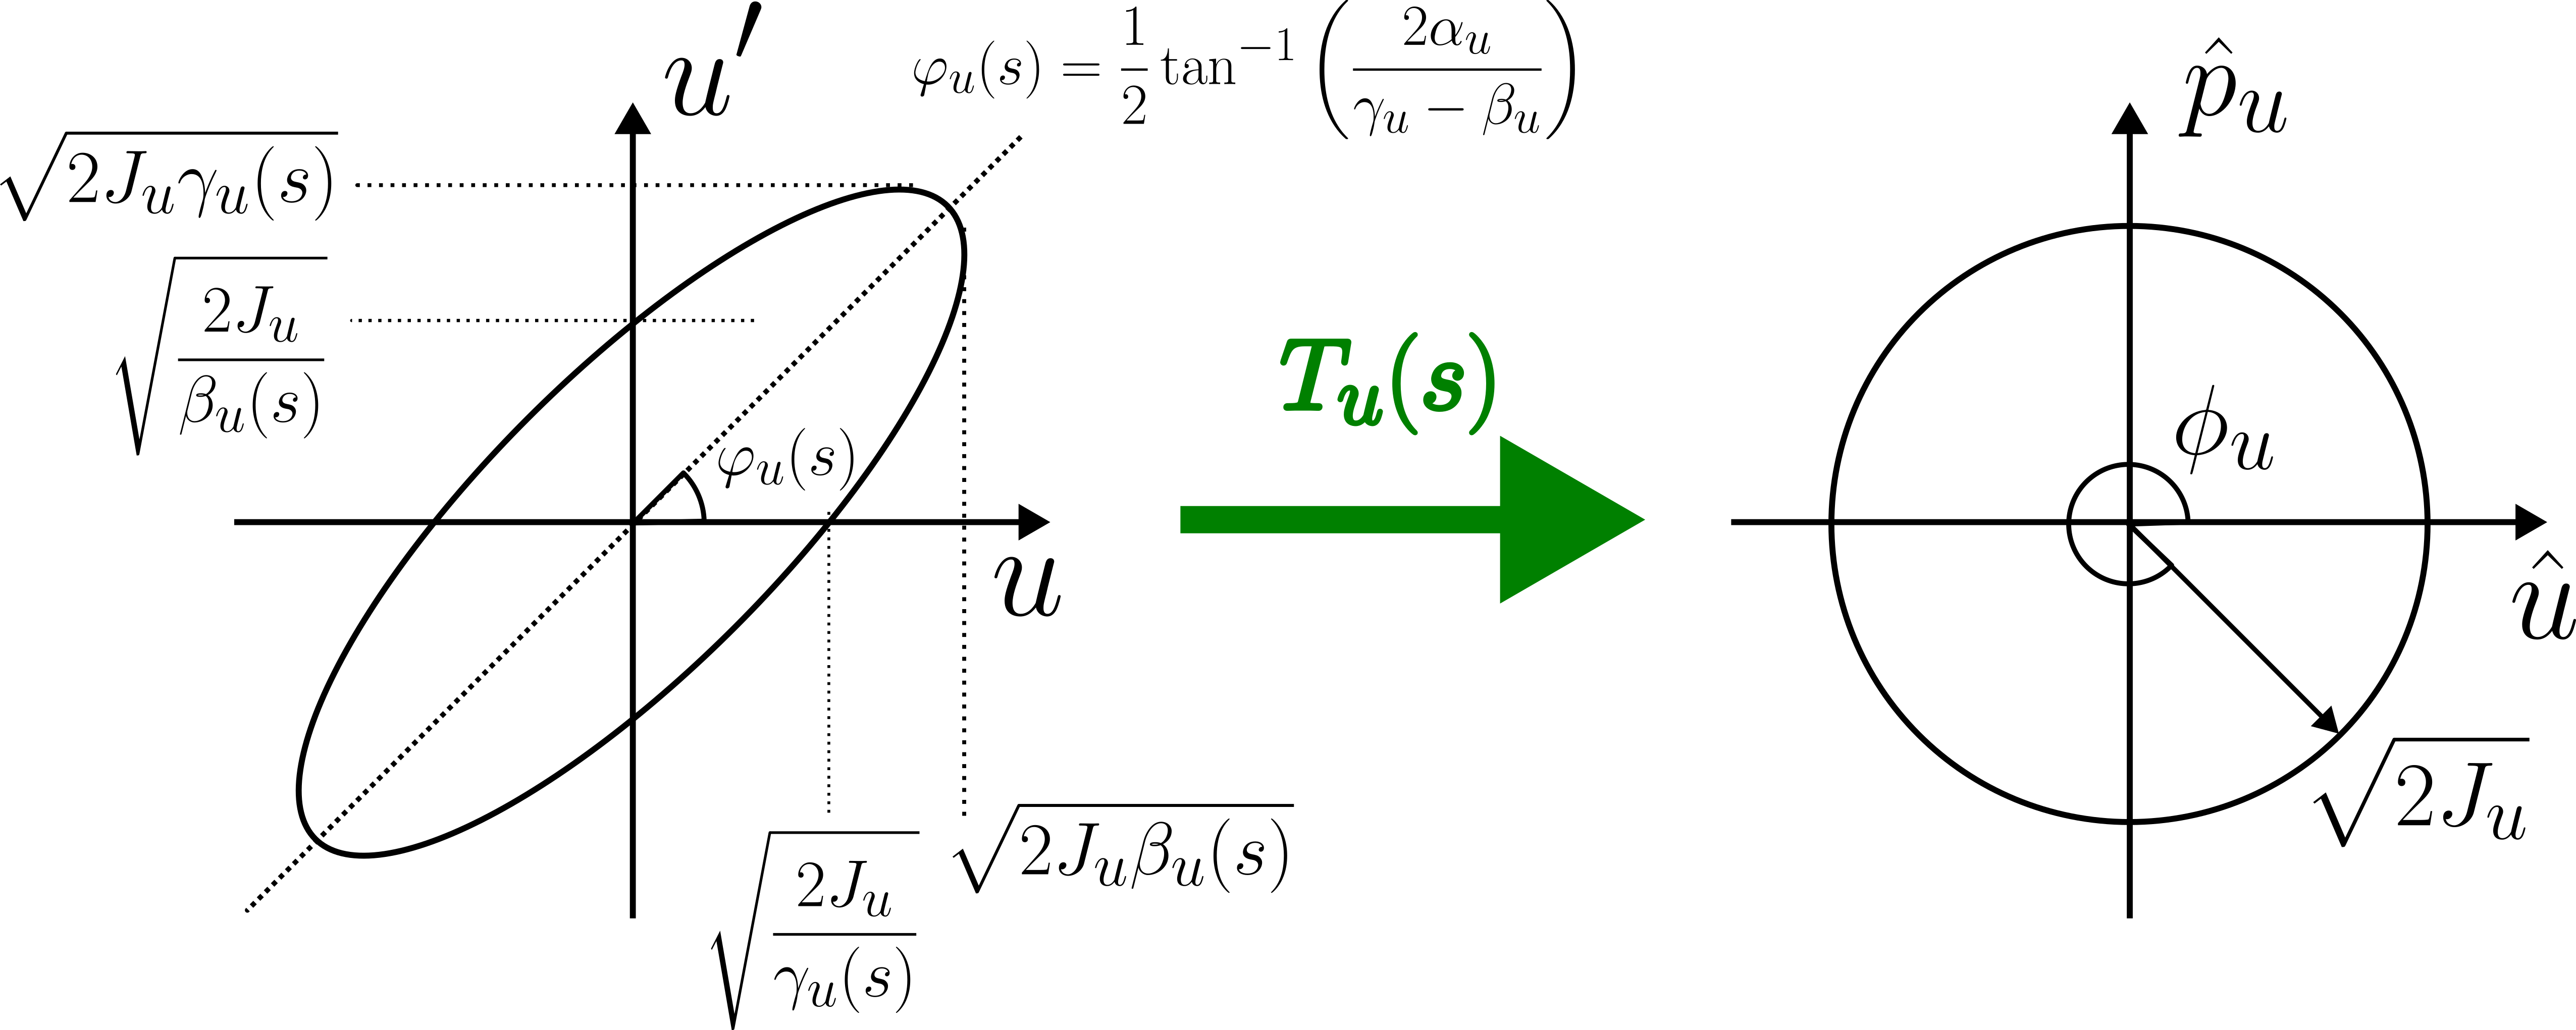
\includegraphics[width=\columnwidth]{chapter2/ellipses.png}
    \caption{Phase space ellipse in geometrical coordinates with Twiss parametrization and its counterpart transformation in normalized phase space.}
    \label{fig:ellipses}
 \end{figure}

Figure \ref{fig:ellipses} also hints at the fact that a linear transformation $T_u(s)$ can be done in order to transform the phase space ellipse into a circle. This is referred to as a Floquet transformation. Therefore, a change of coordinates from geometrical coordinates $(u,u')$ to normalized coordinates $(\hat{u},\hat{p}_u)$ can be achieved through the following linear transformation:
\begin{equation}
    \label{eq:floquet}
    \begin{bmatrix} 
        \hat{u} \\
        \hat{p}_u     
    \end{bmatrix}
    =
    \begin{bmatrix} 
        \frac{1}{\sqrt{\beta_u}} & 0 \\ 
        \frac{\alpha_u}{\beta_u} & \sqrt{\beta_u}
    \end{bmatrix}
    \begin{bmatrix} 
        u \\
        u'     
    \end{bmatrix}
    =
    \sqrt{2J_u}
    \begin{bmatrix} 
        \cos \phi _u (s) \\
        -\sin \phi _u (s)    
    \end{bmatrix}.
\end{equation}
Ultimately, Floquet and his transformations show that the one-turn Hamiltonian for circular accelerators can be expressed as:
\begin{equation}
    \label{eq:hflo}
    H_0=2\pi Q_x J_x + 2\pi Q_y J_y,
\end{equation}
which is simpler and more succinct than the Hamiltonian in Eq. \ref{eq:ham1}. Conclusively, all the dynamics of a linear circular accelerator with all of its intricacies can be mapped to rotations on a simple circle. The dynamics in normalized phase space is just parametrized by a rotation matrix $R(s)$, that will depend on the lattice itself, and is analogous to the transfer matrices $M(s)$ in geometrical space. Therefore, linear dynamics in a circular accelerator can be summarized with the following commutative diagram:      
\begin{equation}\begin{tikzcd}
    {\begin{pmatrix} x,x' \\ y,y' \end{pmatrix}_0} & {} & {\begin{pmatrix} x,x' \\ y,y' \end{pmatrix}_{f}} \\
	\\
	{\begin{pmatrix} J_x,\phi_x \\ J_y,\phi_y \end{pmatrix}_0} & {} & {\begin{pmatrix} J_x,\phi_x \\ J_y,\phi_y \end{pmatrix}_{f}.} \\
	\arrow["{M(s)}", from=1-1, to=1-3]
	\arrow["{T(s)}"', from=1-1, to=3-1]
	\arrow["{R(s)}"', from=3-1, to=3-3]
	\arrow["{T(s)}", from=1-3, to=3-3]
\end{tikzcd}\end{equation}

Before proceeding to the next sections, where Lie operators are introduced in order to generalize to non-linear mappings, a short summary is adequate. For a linear circular accelerator, the last section has shown that starting from Hill's equation, linear transformations can be applied to a complex machine such as an accelerator in order to end up with a simple mathematical equation such as the one described in Eq. \ref{eq:hflo}. Simply put, nonlinear elements will distort the phase space circle of Fig. \ref{fig:ellipses}, destroying the linearity of the system. The premise here is that non-linear elements in circular accelerators are inevitable, and they will come from anywhere and everywhere in the lattice, either from accounted or unaccounted sources. Therefore, higher-tier mathematical tools have to be used in order to describe non-linear dynamics in a circular accelerator. Linear matrices will only get you so far.  

\section{\label{sec:lie}Lie Maps in Accelerator Physics}

The most basic element of a particle accelerator can be thought of as a LEGO® brick acting as a black box transformation for a single particle. This black box takes some single charged particle with initial transverse coordinates $\left( x_0,x'_0,y_0,y'_0 \right)$, as defined in a Frenet-Serret coordinate system, and maps them to some final coordinates $\left( x_f,x'_f,y_f,y'_f \right)$. For simplicity, any longitudinal effect will not be taken into account for this analysis, but can be easily incorporated. By gathering the initial coordinates into a vector, i.e. $\vec{X_0} = \left( x_0,x_0',y_0,y_0' \right)$, and doing the same for the final coordinates, i.e., $\vec{X_f} = \left( x_f,x_f',y_f,y_f' \right)$, one can define the mapping $\mathcal{M}$ that relates both vectors, such that:  
\begin{equation}
\label{eq:ch2map}
\vec{X_f}=\mathcal{M}\vec{X_0}.
\end{equation}
Different from the previous section, $\mathcal{M}$ need not be a linear mapping. For a charged particle inside some accelerator element that can be described using Hamiltonian dynamics, the mapping $\mathcal{M}$ can be understood in terms of Poisson brackets and exponential Lie operators \cite{wolski,todd1,cernthesis1,cernthesis2,forest}.\\
Let $\vec{X} = \left( q_1,p_1,\dots,q_{n},p_{n} \right)$ be a 2n dimensional vector, made from $n$ pairs of canonical coordinates $(q_i,p_i)$ that make up the 2$n$ dimensional phase space. And let two arbitrary functions $f\left( \vec{X};s\right)$ and $g\left( \vec{X};s\right)$ be functions of $\vec{X}$ and $s$, where $s$ plays the role of the independent "time" coordinate. The Poisson brackets $\left[ \bullet , \bullet \right]$ can be defined as:
\begin{equation}
    \label{eq:ch2poisson}
    \left[ f,g \right] = \sum_{i=1}^{n} \frac{\partial f}{\partial q_i}\frac{\partial g}{\partial p_i} - \frac{\partial f}{\partial p_i}\frac{\partial g}{\partial q_i}. 
\end{equation}
Using this definition, one can explicitly write out the Poisson bracket definition for a 4 dimensional phase space described by state vector $\vec{X} = \left( x,x',y,y' \right)$. This reads: 
\begin{equation}
    \label{eq:ch2poisson1}
    \left[ f,g \right] = \frac{\partial f}{\partial x}\frac{\partial g}{\partial x'} - \frac{\partial f}{\partial x'}\frac{\partial g}{\partial x} + \frac{\partial f}{\partial y}\frac{\partial g}{\partial y'} - \frac{\partial f}{\partial y'}\frac{\partial g}{\partial y}. 
\end{equation}\\
The Lie operator $:f:$ acts on some function $g$ and is the adjoint operator of the Poisson bracket operator. Its definition reads:
\begin{equation}
    \label{eq:ch2lie1}
    :f:g = \left[ f,g \right].
\end{equation}
This specific $:\bullet:$ notation allows for a compact notation in order to define the exponential Lie operator. The exponential Lie operator of an arbitrary function $f$ is defined as
\begin{equation}
    \label{eq:ch2explie1}
    e^{:f:}\bullet = \sum_{k=0}^{\infty}\frac{1}{k!}\left( :f: \right)^k \bullet.
\end{equation}
For a Hamiltonian system, the mapping of coordinates from $\vec{X_0}$ to $\vec{X_f}$ follows the expression:
\begin{equation}
    \label{eq:ch2liemap1}
    \vec{X_f}=e^{-\ell :H:}\vec{X}\bigg\rvert_{\vec{X}=\vec{X_0}},
\end{equation}
which is known as a Lie Map \cite{todd1}. In this case, $\ell$ corresponds to the integration length of the independent coordinate. For example, for a particle traversing a magnet which has length $L$, the integration length is $\ell = L$. When looking at the one-turn map, the integration length corresponds to the circumference $C$ of the accelerator over an effective Hamiltonian $H_{eff}$. Furthermore, if working with action-angle variables, the integration length $\ell$ would just be the phase advance $\mu$. An implementation of exponential Lie operators using \textit{Mathematica} \cite{mathematica} in order to calculate 2D and 4D mappings is presented in Appendix \ref{sec:app1} and in Appendix \ref{sec:app2}, respectively.\\ 

\section{\label{sec:oneturn}One-turn Map and Normal Form}

Such as LEGO® bricks can be put together to create complex structures, accelerator elements can be assembled together to create complex ring-shaped structures such as circular accelerators. In such structures, particles will experience the same one-turn mapping over thousands or even millions of turns. The one-turn map $\mathcal{M}_1$ of a circular accelerator is the composition ($\circ$) of mappings from every LEGO® element in the ring. Choosing an arbitrary initial point at $s=0$ and going around the ring, the one-turn map describes the transformation of coordinates after one turn, i.e., $\vec{X}_{N=1}=\mathcal{M}_1 \vec{X_0}$. This map composition reads:
\begin{equation}
    \label{eq:oneturnmap}
    \mathcal{M}_1=M_{N+1} \circ e^{:h_N:} \circ \dots \circ e^{:h_2:} \circ M_2 \circ e^{:h_1:} \circ M_1 = M_{N+1}e^{:h_N:} \dots e^{:h_2:}M_2 e^{:h_1:}M_1,
\end{equation}
where $M_i$ is the matrix representation of a linear mapping, that does not couple $x-y$ plane, e.g., drift space mapping, quadrupole mapping. On the other hand, the map $e^{:h_i:}$ represents any linear or non-linear mapping that can be found around the machine and can be considered a perturbation to the ideal lattice including coupling elements, e.g., skew quadrupoles, higher order multipole elements. Figure \ref{fig:oneturn} illustrates the procedure to build the one-turn map for a circular accelerator. 

\begin{figure}[H]
    \centering
    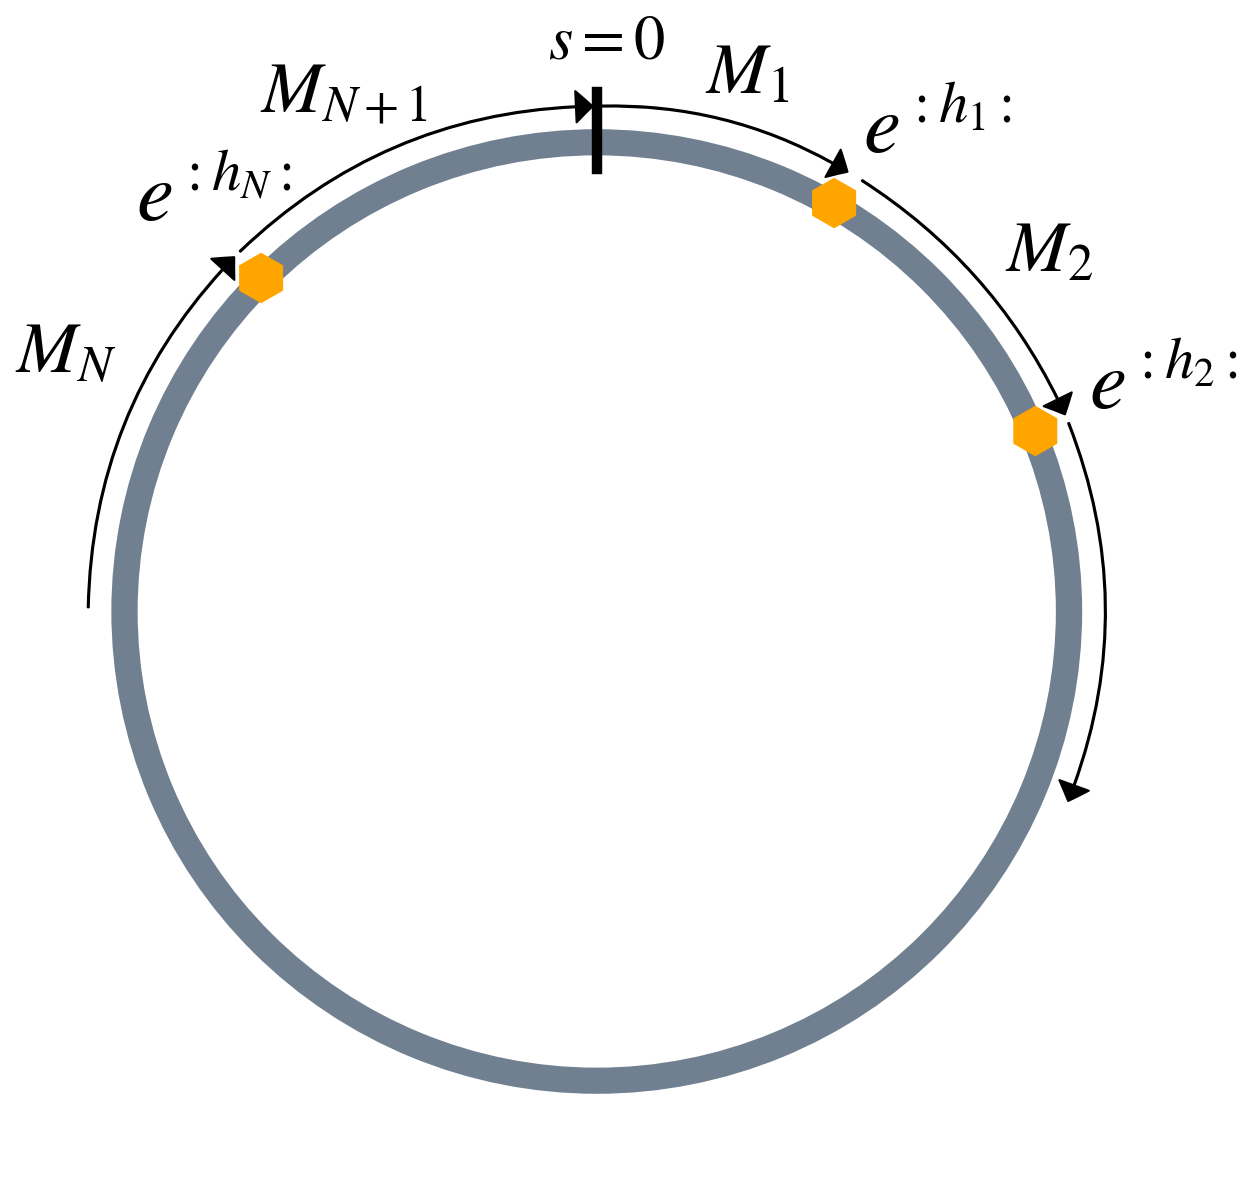
\includegraphics[width=0.7\columnwidth]{chapter2/oneturn.png}
    \caption{Diagram of an arbitrary circular accelerator in order to illustrate the one-turn map.}
    \label{fig:oneturn}
 \end{figure}

Through the use of the Baker-Campbell-Hausdorff formula \cite{bch}, Eq. \ref{eq:oneturnmap} can be collapsed to the expression 
\begin{equation}
    \label{eq:oneturnmapeff}
    \mathcal{M}_1=e^{-C :H_{eff}:},
\end{equation}
where $C$ is the circumference of the ring and $H_{eff}$ is the effective Hamiltonian of the machine over one turn. As mentioned earlier, for most cases, it is of interest to look at the perturbations to the linear uncoupled dynamics of the design lattice. With this in mind, Eq. \ref{eq:oneturnmapeff} can be rewritten as:
\begin{equation}
    \label{eq:oneturnmapeff1}
    \mathcal{M}_1=e^{:h:}R,
\end{equation}
where $R$ is a rotation matrix encoding the linear uncoupled dynamics of the ideal lattice. On the other hand, the term $e^{:h:}$ encodes the perturbations to this ideal situation. It is worth pointing out that for the case $h=0$, the traditional Courant-Snyder variables are recovered.   

The Courant-Snyder variables ($\hat{x}$,$\hat{p}_x$,$\hat{y}$,$\hat{p}_y$) or normalized phase space coordinates can be written for a linear uncoupled case as:
\begin{equation}
    \label{eq:norm1}
    \hat{u}=\sqrt{2J_u} \cos \left( \phi_u + \phi_{u_0}\right);
\end{equation}
\begin{equation}
    \label{eq:norm2}
    \hat{p}_u=-\sqrt{2J_u} \sin \left( \phi_u + \phi_{u_0}\right),
\end{equation}
where $u$ can stand either for the $x$ or $y$ coordinate, $J_u$ and $\phi_u$ correspond to the action-angle variables and $\phi_{u_0}$ corresponds to the initial phase. For the case where perturbations exist, i.e., $h \neq 0$, the action $J_u$ is not constant anymore and will be a function of $\phi_u$.  

The Normal Form formalism is introduced at this point in order to find action-angle coordinates $I_u$ and $\psi_u$, such that the motion just depends on $\psi_u$ at a constant $I_u$, with some initial phase $\psi_{u_0}$. These are known as non-linear action-angle variables. The variables $I_u$ and $\psi_u$ are calculated from the transformation $e^{-:F:}$ acting on $J_u$ and $\phi_u$. The whole point is to find these variables that allow for the Hamiltonian to be only amplitude dependent. These Normal Form gymnastics can be summarized by the following commutative diagram: 

\begin{equation}\begin{tikzcd}
	{\begin{pmatrix} J_x,\phi_x \\ J_y,\phi_y \end{pmatrix}_0} & {} & {\begin{pmatrix} J_x,\phi_x \\ J_y,\phi_y \end{pmatrix}_{f}} \\
	\\
	{\begin{pmatrix} I_x,\psi_x \\ I_y,\psi_y \end{pmatrix}_0} && {\begin{pmatrix} I_x,\psi_x \\ I_y,\psi_y \end{pmatrix}_{f}}
	\arrow["{e^{:h(J_u,\phi_u):}R}", from=1-1, to=1-3]
	\arrow["{e^{-:F:}}"', from=1-1, to=3-1]
	\arrow["{e^{:H(I_u):}}"', from=3-1, to=3-3]
	\arrow["{e^{-:F:}}", from=1-3, to=3-3]
    .
\end{tikzcd}\end{equation}

Without loss of generality, the generating function $F$ can be written as a Fourier expansion over the objective space $(I_x,\psi_x,I_y,\psi_y)$ such that:
\begin{equation}
    \label{eq:F}
    F=\sum_{jklm} f_{jklm} \left( 2 I_x\right)^{\frac{j+k}{2}} \left( 2 I_y\right)^{\frac{l+m}{2}} e^{i\left[ \left( j-k \right)\left( \psi_x+\psi_{x0} \right)+ \left( l-m \right) \left( \psi_y+\psi_{y0} \right)\right]}.
\end{equation}
Similarly, the argument of the Lie operator $e^{:h:}$ from Eq. \ref{eq:oneturnmapeff1} can be expanded as:
\begin{equation}
    \label{eq:h}
    h=\sum_{jklm} h_{jklm} \left( 2 J_x\right)^{\frac{j+k}{2}} \left( 2 J_y\right)^{\frac{l+m}{2}} e^{i\left[ \left( j-k \right)\left( \phi_x+\phi_{x0} \right)+ \left( l-m \right) \left( \phi_y+\phi_{y0} \right)\right]}.
\end{equation}
For Eqs. \ref{eq:F} and \ref{eq:h}, the integer indices $j,k,l,m$ run from $0$ to infinity, and correspond to the four degrees of freedom for transverse phase space.   

The terms $f_{jklm}$ are known as generating function coefficients. The terms $h_{jklm}$ are known as Hamiltonian coefficients or resonance driving terms (RDTs). Section \ref{sec:rdts} will take a closer look into how RDTs can be used to characterize the non-linear dynamics of accelerators. The generating function coefficients $f_{jklm}$ can be related to the Hamiltonian resonance driving terms $h_{jklm}$ through the following relation \cite{cernthesis1,bartolini}:
\begin{equation}
    \label{eq:handf}
    f_{jklm}=\frac{h_{jklm}}{1-e^{2\pi i \left[ \left( j-k \right) Q_x + \left( l-m\right) Q_y \right] }},
\end{equation}
where $Q_x$ and $Q_y$ represent the transverse uncoupled and unperturbed tunes of the accelerator. The transverse tunes of a circular accelerator are defined as the phase advances in each plane over one turn, in units of $2\pi$, i.e., $Q_u=\phi_u(s=C)/2\pi$. 

In general, the terms $h_{jklm}$ are defined by the order in which they enter the one-turn normal form Hamiltonian \cite{bartolini}. With the assumption of thin elements around the ring, the general expression to define RDTs reads:
\begin{equation}
    \label{eq:rdt1}
    h_{jklm}=\Xi _{jklm} \sum_i L_i K_{n-1,i} \beta_{x,i}^{\frac{j+k}{2}} \beta_{y,i}^{\frac{l+m}{2}} e^{i\left[ (j-k)\phi_{x,i} +(l-m) \phi_{y,i} \right]},
\end{equation}
where $\Xi _{jklm}$ is just a constant defined as:
\begin{equation}
    \label{eq:rdt2}
    \Xi _{jklm} = -\frac{1}{2^n}\frac{1}{n!} {\binom{n}{l+m}} {\binom{j+k}{j}}{\binom{l+m}{l}}.
\end{equation}

For Eqs. \ref{eq:rdt1} and \ref{eq:rdt2}, $n=j+k+l+m$ represents the order of the RDT. The sum over $i$ is done over all multipoles of order $n$ and length $L_i$ that either have a normal component $K_{n-1,i}=b_{n-1,i}/\rho$ if $l+m$ is even, or a skew component $K_{n-1,i}= K_{n-1,i}^{(s)}= a_{n-1,i}/\rho$ if $l+m$ is odd, remembering $\rho$ is the bending radius as it appeared on Eq. \ref{eq:ch2magnet}. The notation $K_{n-1,i}$ is to keep up with the MAD-X convention for naming normal multipole coefficients \cite{madx}. The symbols for $\beta_{x,i}$, $\beta_{y,i}$, $\phi_{x,i}$ and $\phi_{y,i}$ represent the unperturbed beta functions and phase advances in each plane, respectively.

\section{\label{sec:resonances}Resonances in Circular Accelerators}

Equation \ref{eq:handf} diverges for when the denominator goes to zero. Specifically, this happens when the following condition is met:
\begin{equation}
    \label{eq:resonances}
    \left( j-k \right) Q_x + \left( l-m\right) Q_y = p,
\end{equation}
where $p$ can be any integer. Equation \ref{eq:resonances} defines resonance lines in tune space of order $n=j+k+l+m$. If the accelerator is tuned to operate on top of these resonances, the perturbations will add up coherently turn to turn and kick the resonant particles out of their original trajectory. In general, operating close or on top of a resonance line is harmful as particles will be lost. This is specially true for lower order resonances, i.e., for $n<4$. In general, the higher order of a resonance, the weaker it is \cite{Wiedemann2015}. This thesis work focuses on third order resonances, i.e., $n=3$, and how to mitigate their deleterious effect. 

Figure \ref{fig:tunediagram} shows the tune diagram with resonance lines, as defined by Eq. \ref{eq:resonances}, drawn up to fifth order. The integer part of both tunes are chosen to include the actual area of operation of the Recycler Ring. Nevertheless, only the fractional part of the tune carries the significant information for resonance diagrams. The operation and tune diagram for the Recycler Ring are described in more detail in Ch. \ref{sec:ch3}. Normally, the operation point of a circular accelerator is chosen to be clear of any resonance line and far away as possible from integer ($n=1$) and half integer ($n=2$) resonances. Nevertheless, in reality there are two concepts that complicate things. The first one relates to the fact that resonance lines are not infinitely thin and have some stop bandwidth. The second one, concerns the fact that at high intensities particles will not have localized tunes, but rather a distribution of tunes with some tune spread, i.e., a tune footprint. Section \ref{sec:sc1} takes a closer look at this effect known as space charge tune shift. Ultimately, choosing the operation point on Fig. \ref{fig:tunediagram} is a matter of localizing a resonance-free region where the intensity-dependent tune footprint can be placed.   
\begin{figure}[H]
    \centering
    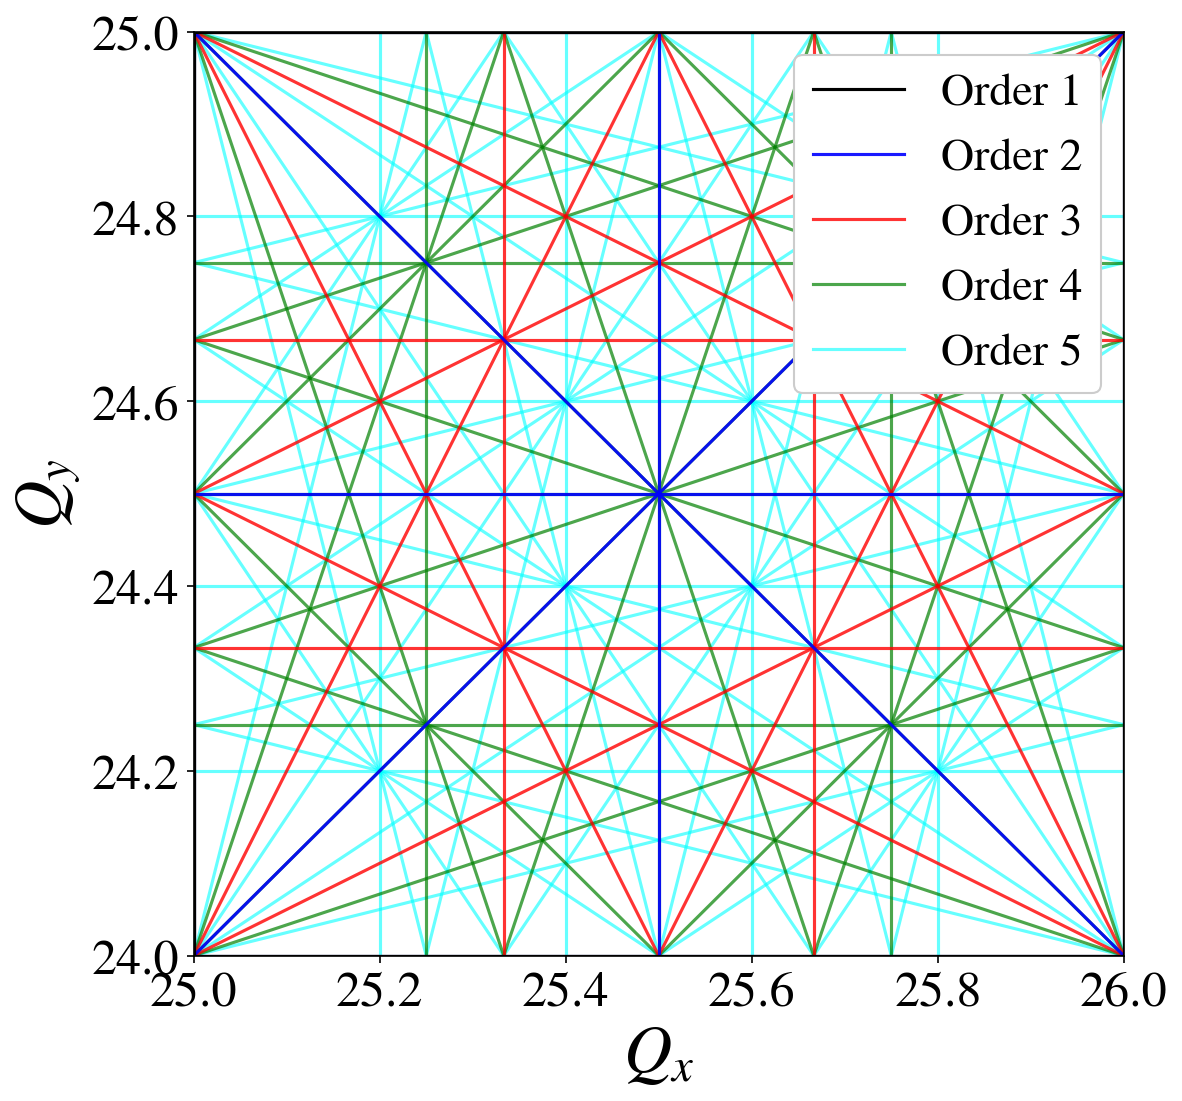
\includegraphics[width=0.8\columnwidth]{chapter2/tunediagram.png}
    \caption{Tune diagram with resonance lines up to fifth order, enclosing the operation point of the Recycler Ring.}
    \label{fig:tunediagram}
 \end{figure}
It is worth stopping here and asking what is the driving force behind each of these resonance lines. Classic accelerator references such as Refs. \cite{wolski,Wiedemann2015,sylee} will derive Eq. \ref{eq:resonances} by perturbing Hill's equation with different magnetic multipole orders. A closer look into each perturbation term reveals that half integer resonances are caused by quadrupole terms, third order resonances by sextupole-like terms, fourth order resonances by octupole terms, and so on and so forth. Nevertheless, the story complicates when one takes into account that pure multipole magnets can feed down or up to other order terms if there is installation misalignment, e.g., a misaligned sextupole feeds to skew quadrupole-like terms.        

Figure \ref{fig:rrtdlow} zooms into the region of interest for the Recycler Ring operation in the tune diagram, as shown in Fig. \ref{fig:tunediagram}. As mentioned before, the operation point of an accelerator in the tune diagram is not a singular point but rather a footprint. While the lattice can be tuned to a specific nominal point, particles will interact with other particles through the Coulomb force. Consequently, each particle will feel a different tune shift depending on their position within the bunch of particles. This is called the incoherent space charge tune shift, and it will be the largest for particles in the core of the bunch, i.e., the beam core. At low particle intensities, such as the one used to produce Fig. \ref{fig:rrtdlow}, the tune spread of the particles in the bunch is small enough to approximate the physics to single-particle dynamics. For beams with low particle intensities and a small tune spread, such as the one depicted in Fig. \ref{fig:rrtdlow}, operating clear from any low order resonance lines is not generally a problem. Nevertheless, at high intensities the situation changes.   

 \begin{figure}[H]
    \centering
    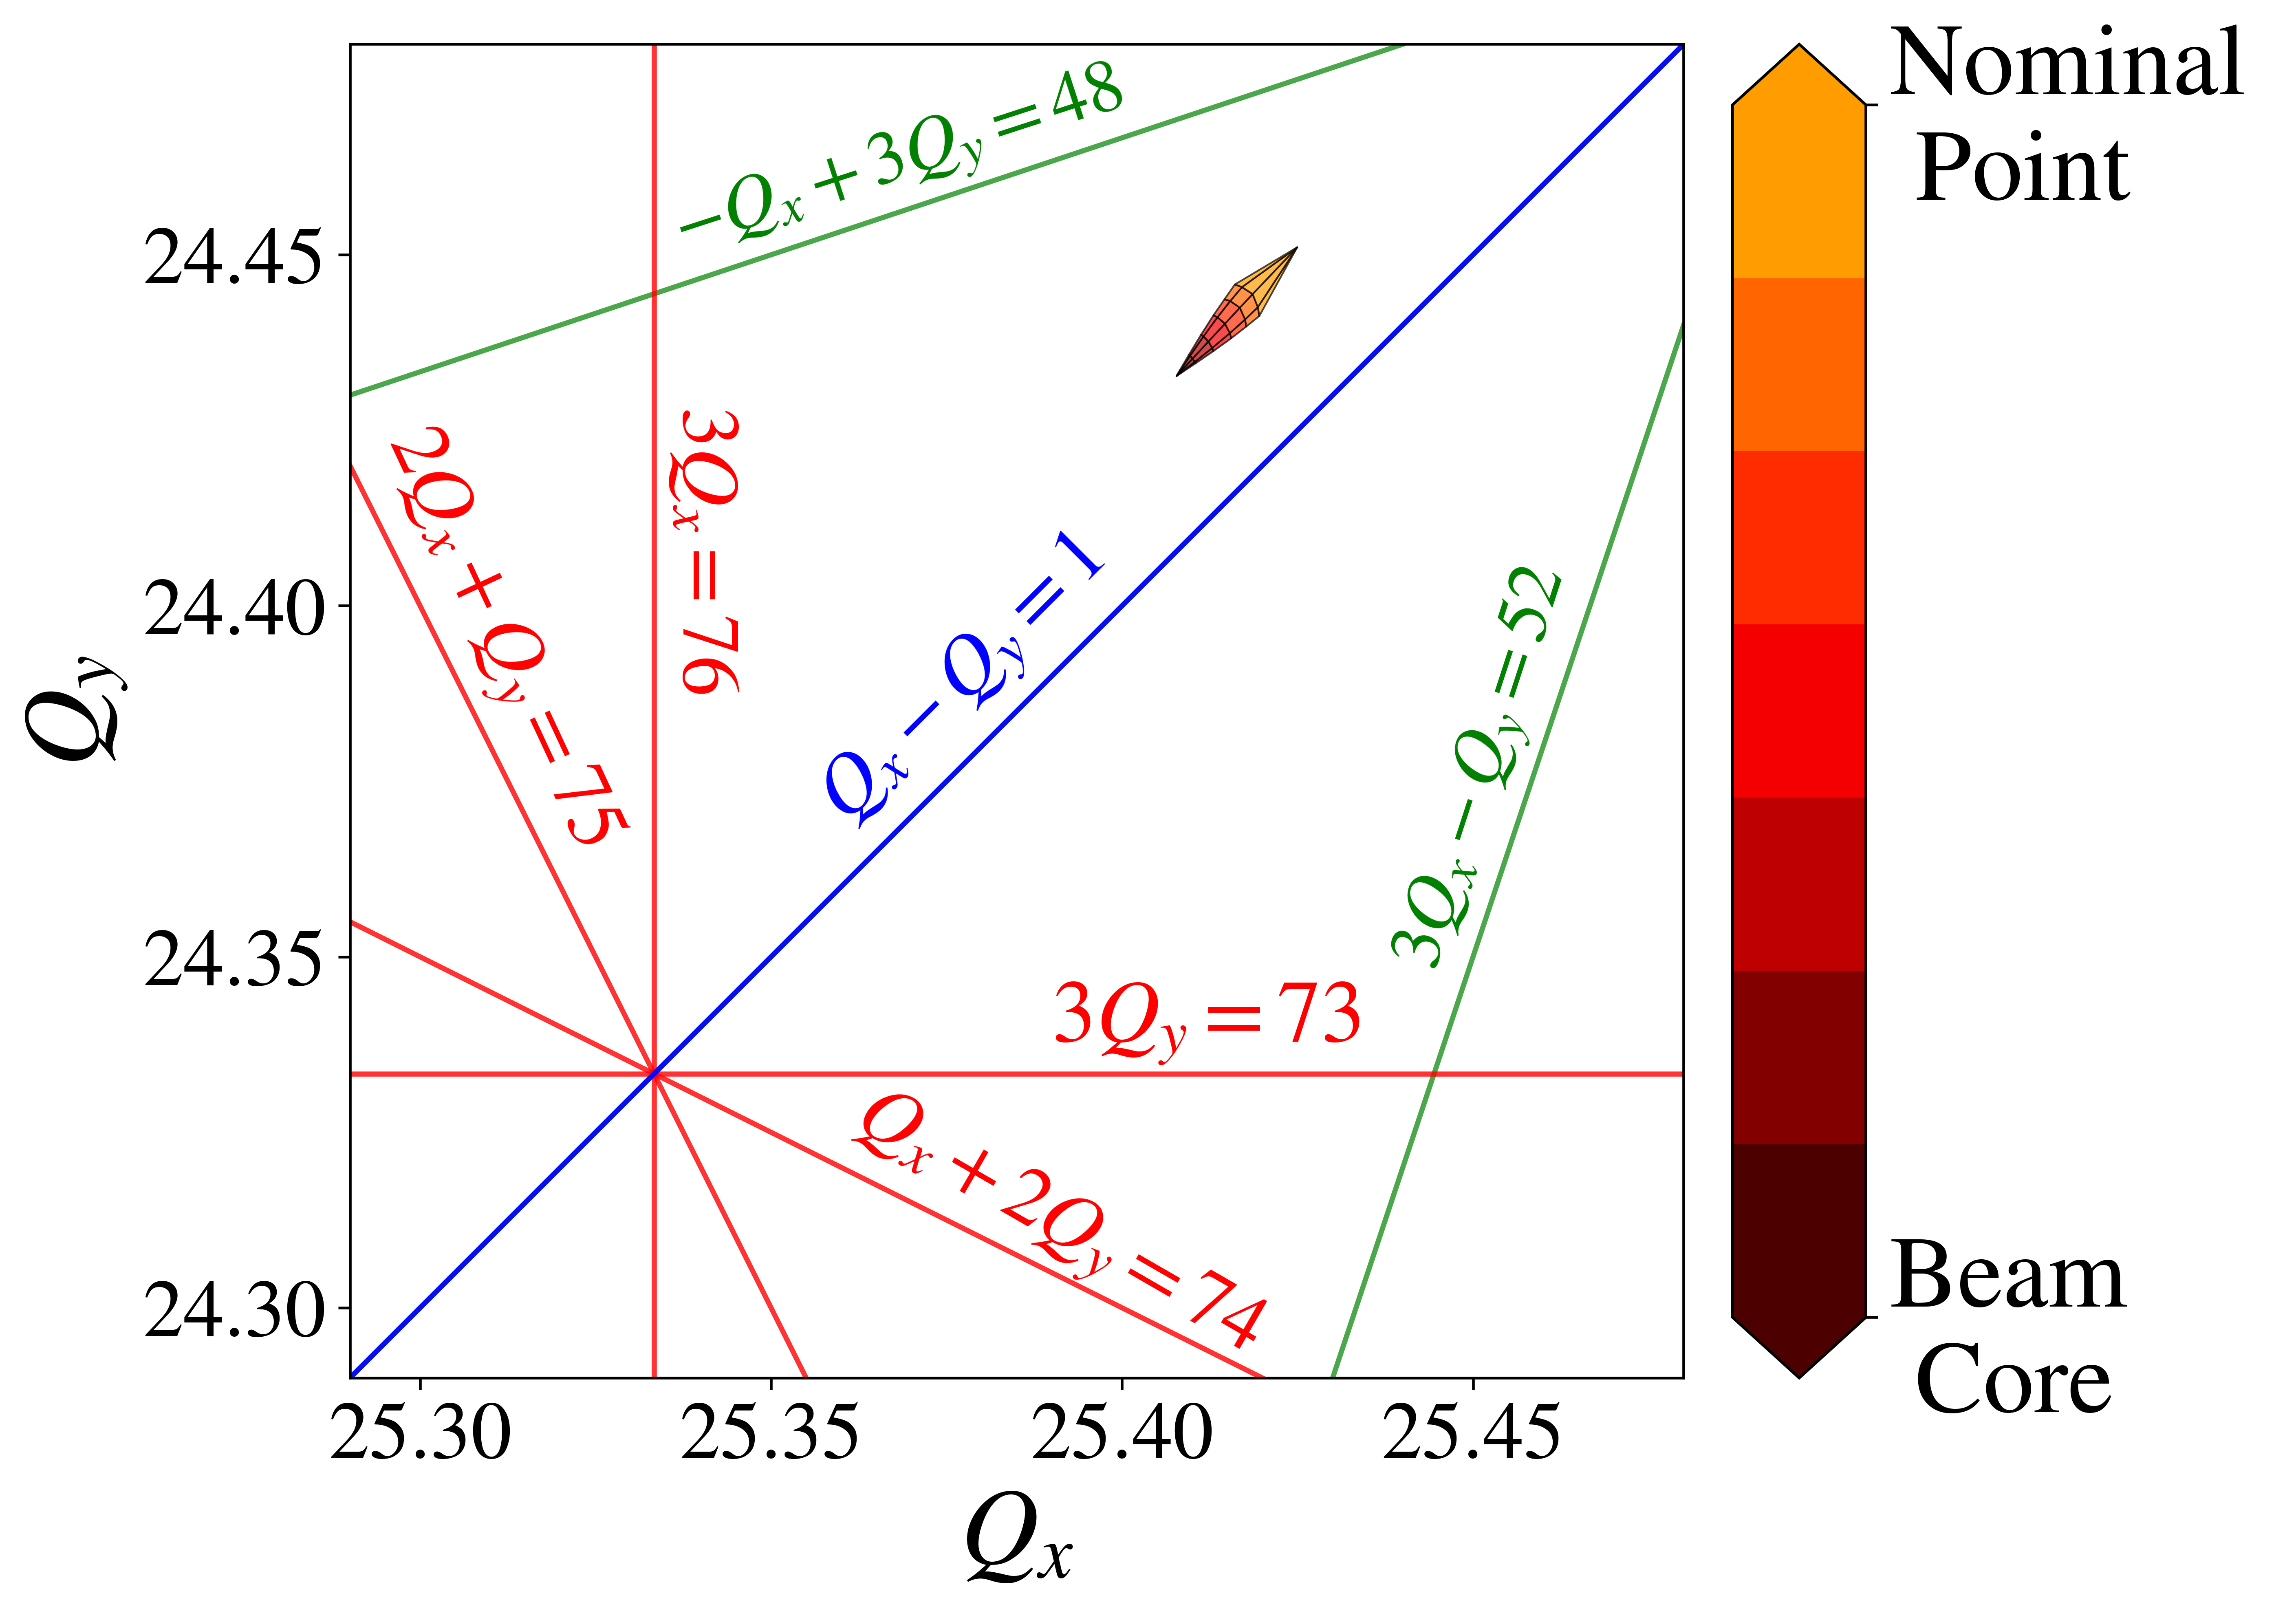
\includegraphics[width=\columnwidth]{chapter2/rrtdlow.png}
    \caption{Approximate operational tune footprint at low intensities calculated with PySCRDT \cite{pyscrdt}, i.e., 1e10 particles per bunch.}
    \label{fig:rrtdlow}
 \end{figure}

Figure \ref{fig:rrtdlow} plots all resonance lines up to fourth order in this region of interest. The half integer line $Q_x-Q_y=1$, also known as a difference coupling resonance, is usually driven by solenoidal and skew-quadrupole fields in the lattice. The third order lines $3Q_x=76$ and $Q_x+2Q_y=74$ are driven by sextupole-like fields. The other third order lines $3Q_y=73$ and $2Q_x+Q_y=75$ are driven by skew sextupole terms in the lattice. And finally, the fourth order lines $-Q_x+3Q_y=48$ and $3Q_x-Q_y=52$ are driven by octupole terms in the lattice and Coulomb (space charge) forces from the bunch itself. This is assuming a rectangular multipole expansion notation of the magnetic field, such as the one presented in Eq. \ref{eq:ch2magnet}.      

\section{\label{sec:rdts}Resonance Driving Terms} 

The RDTs $h_{jklm}$ are related to the strength of the resonance $\left( j-k \right) Q_x + \left( l-m\right) Q_y$. Therefore, controlling and measuring these RDTs is of special interest to accelerator physics. The following section explains how to get to a useful expression that can be used in order to measure the $h_{jklm}$ terms through Fourier expansions.

The whole point of introducing the Normal Form coordinates ($I_u,\psi_u$) through the transformation $e^{-:F:}$ as defined in Eq. \ref{eq:F} is to transfer complicated non-linear dynamics to simple dynamics that lie on a circle where the action is conserved $I_u$ and $\dot{\psi_u}$ is constant. When this happens, a set of canonical coordinates $\vec{\zeta} = \left( \zeta_x^+ , \zeta_x^-, \zeta_y^+, \zeta_y^-\right)$ can be defined as:
\begin{equation}
    \label{eq:zeta}
    \zeta_u^{\pm}=\sqrt{2I_u}e^{\mp i\left( \psi_u + \psi_{u_0}\right)},
\end{equation}
always keeping in mind that $I_u$ is a constant of motion and $\psi_{u_0}$ is a constant initial phase set by the initial conditions. It can be shown that the Poisson brackets for a pair of these quantities are:
\begin{equation}
    \label{eq:zetapoisson}
    \left[ \zeta_u^{+}, \zeta_u^{-} \right]_{\psi_u,J_u} = \frac{\partial \zeta_u^{+}}{\partial \psi_u}\frac{\partial \zeta_u^{-}}{\partial J_u} - \frac{\partial \zeta_u^{+}}{\partial J_u}\frac{\partial \zeta_u^{-}}{\partial \psi_u}=-2i,
\end{equation}
for the same plane $u$ and using a reduced form of Eq. \ref{eq:ch2poisson1}. In this notation, the subindices from $[\bullet,\bullet]_{\psi_u,J_u}$ refer to the variables to be used in order to calculate the Poisson brackets. Using Eq. \ref{eq:zetapoisson}, the following useful property can be derived:
\begin{equation}
    \label{eq:zetapoisson2}
    \left[ {\zeta_x^{+}}^j {\zeta_x^{-}}^k {\zeta_y^{+}}^l {\zeta_y^{-}}^m, \zeta_x^{-} \right]_{\psi_x,J_x} = \left( {\zeta_y^{+}}^l {\zeta_y^{-}}^m \right)\left[ {\zeta_x^{+}}^j {\zeta_x^{-}}^k, \zeta_x^{-} \right]_{\psi_x,J_x} =-2ij {\zeta_x^{+}}^{j-1} {\zeta_x^{-}}^k {\zeta_y^{+}}^l {\zeta_y^{-}}^m ,
\end{equation}   
where the last step can be achieved using Leibnitz rule for Poisson brackets, i.e., $[fg,h]=[f,h]g+f[g,h]$.

On the other hand, going back to the Courant-Snyder phase space, a set of coordinates known as a resonance basis $\vec{h} = \left( h_x^+ , h_x^-, h_y^+, h_y^-\right)$ can be defined. Similarly to Eq. \ref{eq:zeta}, the resonance basis reads:
\begin{equation}
    \label{eq:hbasis}
    h_u^{\pm}=\hat{u}\pm \hat{p}_u=\sqrt{2J_u}e^{\mp i\left( \phi_u + \phi_{u_0}\right)},
\end{equation}
always keeping in mind that in the Courant-Snyder phase space, the action $J_u$ is a function of the phase $\phi_u$, i.e., $J_u = J_u(\phi_u)$ and is not constant. The initial phase $\phi_{u_0}$ is again a constant set by the initial conditions. 

The basis grouped in $\vec{h}$ and the one grouped in $\vec{\zeta}$ are related by the transformation:
\begin{equation}
    \label{eq:htozeta}
    \vec{h}=e^{:F \left(\vec{\zeta}\right):}\vec{\zeta},
\end{equation}
where $F(\vec{\zeta})$ is the generating function written in terms of the basis $\vec{\zeta}$. The inverse transformation to Eq. \ref{eq:htozeta} reads:
\begin{equation}
    \label{eq:zetatoh}
    \vec{\zeta}=e^{-:F\left( \vec{\zeta} \right):}\vec{h}.
\end{equation}
Writing out the generating function $F(\vec{\zeta})$ in a general polynomial form, this functions reads:
\begin{equation}
    \label{eq:Fzeta}
    F\left( \vec{\zeta} \right)=\sum_{jklm} f_{jklm} {\zeta_x^{+}}^{j} {\zeta_x^{-}}^k {\zeta_y^{+}}^l {\zeta_y^{-}}^m.
\end{equation}
By inserting the definitions in Eq. \ref{eq:zeta} into Eq. \ref{eq:Fzeta}, the proposed definition in Eq. \ref{eq:F} can be recovered.

Expanding Eq. \ref{eq:htozeta} by using the exponential Lie operator definition from Eq. \ref{eq:ch2explie1} reads:
\begin{equation}
    \label{eq:htozetaexpansion}
    \vec{h}=\vec{\zeta}+\left[ F \left(\vec{\zeta}\right), \vec{\zeta}\right]+\frac{1}{2} \left[ F \left[ F , \vec{\zeta}\right] \right] + \dots,
\end{equation}
where this expression was truncated to second order in the Poisson brackets. By taking only the first two terms of the expansion, and introducing the expression from Eq. \ref{eq:Fzeta}, one can find an approximated expression for $h_{x}^{-}$ which reads:
\begin{equation}
    \label{eq:htozeta2}
    h_x^- \approx \zeta_x^{-} + \left[ F \left(\vec{\zeta}\right), \zeta_x^{-}\right] =  \zeta_x^{-} + \sum_{jklm} f_{jklm} \left[ {\zeta_x^{+}}^{j} {\zeta_x^{-}}^k {\zeta_y^{+}}^l {\zeta_y^{-}}^m, \zeta_x^{-}\right],
\end{equation}
At this point is where the usefulness of Eq. \ref{eq:zetapoisson2} comes into play. Introducing the explicit result from Eq. \ref{eq:zetapoisson2} into Eq. \ref{eq:htozeta2} yields the following expression:
\begin{equation}
    \label{eq:htozeta3}
    h_x^- \approx \zeta_x^{-} -2i \sum_{jklm}j f_{jklm} {\zeta_x^{+}}^{j-1} {\zeta_x^{-}}^k {\zeta_y^{+}}^l {\zeta_y^{-}}^m.
\end{equation}
Manipulating this expression further, the definition for $\zeta_u$ as described in Eq. \ref{eq:zeta} can be introduced into Eq. \ref{eq:htozeta3}. This yields:
\begin{multline}
    \label{eq:hxpsi}
    h_x^{-}(N)=\sqrt{2I_x}e^{i\left( \psi_x+\psi_{x_0}\right)} \\
    -2i \sum_{jklm} j f_{jklm} \left( 2I_x \right)^{\frac{j+k-1}{2}}\left( 2I_y \right)^{\frac{l+m}{2}}
    e^{i \left[ \left( 1-j+k\right)\left( \psi_x + \psi_{x_0} \right) +\left( m-l\right)\left( \psi_y + \psi_{y_0} \right)\right]}.
\end{multline}
At this point, Eq. \ref{eq:hxpsi} is starting to look as a useful Fourier expansion. Ultimately, the data that can be extracted from a circular accelerator will come from a diagnostic device triggered every turn, i.e., turn-by-turn data. For that reason, it will be useful to rewrite Eq. \ref{eq:hxpsi} in terms of the $N$ number of turns of particles in the accelerator. The expression relating the phase advances to the turn number reads:
\begin{equation}
    \label{eq:psiu}
    \psi_u=2 \pi Q_u N, 
\end{equation}  
where $2 \pi Q_u$ is the respective phase advance over one turn of the accelerator, i.e. the tune of the circular accelerator.

Therefore, the resonance basis can be built by getting the quantity $h_u^{\pm}=\hat{u}\pm \hat{p}_u$ in terms of the number of turns $N$ and using Eq. \ref{eq:psiu}. Specifically, for $h_x^{-}$ this reads:
\begin{multline}
    \label{eq:hx-}
    h_x^{-}(N)=\sqrt{2I_x}e^{i\left( 2\pi Q_x N +\psi_{x_0}\right)} \\
    -2i \sum_{jklm} j f_{jklm} \left( 2I_x \right)^{\frac{j+k-1}{2}}\left( 2I_y \right)^{\frac{l+m}{2}}
    e^{i \left[ \left( 1-j+k\right)\left( 2\pi Q_x N + \psi_{x_0} \right) +\left( m-l\right)\left( 2\pi Q_y N + \psi_{y_0} \right)\right]},
\end{multline}
where $Q_x$ and $Q_y$ are the horizontal and vertical uncoupled tune. Note that this analysis can be easily extended to calculate the other elements in $\vec{h}$. These calculations are left as an exercise for the reader.  

\section{\label{sec:amp}Amplitude-Dependent Tune Shift}
The RDT formalism allows to calculate an important quantity in accelerator physics called the amplitude-dependent tune shift. The Hamiltonian for a single particle in a linear circular lattice with perturbation elements reads: 
\begin{equation}
    \label{eq:hh}
    H(x,y,s)=H_{0}(J_x,J_y)+H_{1}(J_x, \phi_x, J_y, \phi_y), 
\end{equation} 
where $H_0$ is the unperturbed linear Hamiltonian with tunes $Q_x$ and $Q_y$, and $H_1$ is the perturbation Hamiltonian stemming from linear and non-linear unaccounted blocks in the lattice.

From Secs. \ref{sec:basic} and \ref{sec:oneturn}, the expressions for $H_0$ and $H_1$ have been explicitly written in Eqs. \ref{eq:hflo} and \ref{eq:h} in terms of $J_x,\phi_x,J_y,\phi_y$, therefore the sum of both expression reads:
\begin{equation}
    \label{eq:h0h1}
    H_0+H_1=2\pi Q_x J_x + 2\pi Q_y J_y + \sum_{jklm} h_{jklm} \left( 2 J_x\right)^{\frac{j+k}{2}} \left( 2 J_y\right)^{\frac{l+m}{2}} e^{i\left[ \left( j-k \right)\left( \phi_x+\phi_{x0} \right)+ \left( l-m \right) \left( \phi_y+\phi_{y0} \right)\right]}.
\end{equation}
Nevertheless, it is important to remember that $H_1$ is the compilation of all perturbations after one turn to the linear Hamiltonian $H_0$, and is therefore perturbative. 

Consequently, for Eq. \ref{eq:h0h1}, the independent time variable is the number of turns $N$. For this case, the equations of motion taking $N$ as the number of turns around the circular accelerator are just:
\begin{equation}
    \label{eq:eom1}
    \frac{\partial J_u}{\partial N} = -\frac{\partial H}{\partial \phi_u} = -\frac{\partial H_1}{\partial \phi_u},
\end{equation}
and
\begin{equation}
    \label{eq:eom2}
    \frac{\partial \phi_u}{\partial N} = \frac{\partial H}{\partial J_u} = 2\pi Q_u + \frac{\partial H_1}{\partial J_u}.
\end{equation}
This last term ${\partial H_1}/{\partial J_u}$ in Eq. \ref{eq:eom2} will define the amplitude-dependent tune shift. If the whole lattice were just a linear lattice, the betatron oscillations would just gain a phase change of $2\pi Q_u$ every turn, i.e., $\Delta \phi(N)=2\pi Q_u N$. Nevertheless, given that this new term $H_1$ perturbs the dynamics in the accelerator, the phase change will now depend on the amplitude $J_u$ of the betatron oscillations of the single particle. Therefore, given that this effect acts on each individual particle, it is an incoherent effect. The effective result from this new term is to detune the circular lattice from its original tune $Q_u$ for each individual particle.

Explicitly calculating the expression from Eq. \ref{eq:eom2} for $J_x$ and $\phi_x$ using the Hamiltonian in Eq. \ref{eq:hh} yields
\begin{equation}
    \label{eq:detune}
    \frac{\partial \phi_x}{\partial N} = 2\pi Q_x + \sum_{jklm} h_{jklm} \left( j+k \right) \left( 2 J_x\right)^{\frac{j+k}{2}-1} \left( 2 J_y\right)^{\frac{l+m}{2}} e^{i\left[ \left( j-k \right)\left( \phi_x+\phi_{x0} \right)+ \left( l-m \right) \left( \phi_y+\phi_{y0} \right)\right]}.
\end{equation}   
In particular, it is of interest to look at the average limit where particles have undergone large number of turns around the circular accelerator $N \rightarrow \infty$. This is done in order to wash out any oscillatory behavior in ${\partial H_1}/{\partial J_u}$. Therefore, the following quantity is of interest: 
\begin{equation}
    \label{eq:Nave1}
    \lim_{N\to\infty} \left\langle \frac{\partial \phi_x}{\partial N}\right\rangle _N = \lim_{N\to\infty} \frac{1}{N} \int_0^N dN' \; {\frac{\partial \phi_x}{\partial N'}},
\end{equation}
which is just the definition for the average of ${\partial \phi_x}/{\partial N}$ over $N$ turns, for many turns. Explicitly calculating this quantity gives:
\begin{multline}
    \label{eq:Nave2}
    \lim_{N\to\infty} \left\langle \frac{\partial \phi_x}{\partial N}\right\rangle _N = 2\pi Q_x\\
    +\sum_{jklm} h_{jklm} \left( j+k\right) \lim_{N\to\infty} \frac{1}{N} \int_0^N dN' \; \left( 2 J_x\right)^{\frac{j+k}{2}-1} \left( 2 J_y\right)^{\frac{l+m}{2}} e^{i\left[ \left( j-k \right)\left( \phi_x+\phi_{x0} \right)+ \left( l-m \right) \left( \phi_y+\phi_{y0} \right) \right]}.
\end{multline}
In general, it is known that $J_u,\phi_u$ depend on the number of turns, i.e., $J_u,\phi_u=J_u (N),\phi_u (N)$. Nevertheless, Eq. \ref{eq:Nave2} can be approximated by inserting the unperturbed solution of $H_0$ which means that $J_u$ is constant and $\phi_u = 2 \pi Q_u N$. With this in mind and assuming the constants $\phi_{u0}=0$ without loss of generality, Eq. \ref{eq:Nave2} reduces to
\begin{multline}
    \label{eq:Nave3}
    \lim_{N\to\infty} \left\langle \frac{\partial \phi_x}{\partial N}\right\rangle _N = 2\pi Q_x\\
    +\sum_{jklm} h_{jklm} \left( j+k \right) \left( 2 J_x\right)^{\frac{j+k}{2}-1} \left( 2 J_y\right)^{\frac{l+m}{2}} \lim_{N\to\infty} \frac{1}{N} \int_0^N dN' \;  e^{2 \pi i \left[ \left( j-k \right) Q_x+ \left( l-m \right) Q_y \right] N'}.
\end{multline}
A closer look into the integral in Eq. \ref{eq:Nave3} reveals that this integral in the limit where $N \rightarrow \infty$ is just a delta function reading $\delta\left( (j-k)Q_x+(l-m)Q_y\right)$. As a reminder, the RDT approximation breaks down if Eq. \ref{eq:resonances} holds. Therefore, it can be shown that the argument in the delta function can only be zero if $j=k$ and $l=m$. Thus, this delta function effectively becomes two Kronecker deltas---$\delta_{jk}$ and $\delta_{lm}$. Inserting this into Eq. \ref{eq:Nave3} yields:
\begin{equation}
    \label{eq:Nave4}
    \lim_{N\to\infty} \left\langle \frac{\partial \phi_x}{\partial N}\right\rangle _N = 2\pi Q_x\\
    +\sum_{jklm} h_{jklm} \left( j+k \right) \left( 2 J_x\right)^{\frac{j+k}{2}-1} \left( 2 J_y\right)^{\frac{l+m}{2}} \delta _{jk} \delta_{lm}.
\end{equation}
Reducing this expression further with the properties of Kronecker deltas reads:
\begin{equation}
    \label{eq:Nave5}
    \lim_{N\to\infty} \left\langle \frac{\partial \phi_x}{\partial N}\right\rangle _N = 2\pi Q_x\\
    +2\sum_{jl} h_{jjll} j \left( 2 J_x\right)^{j-1} \left( 2 J_y\right)^{l}.
\end{equation}
Equation \ref{eq:Nave5} is stating that the constant detuning terms in the accelerators will be given by the terms where $j=k$ and $l=m$. As a consequence of Eq. \ref{eq:rdt1}, for this case the RDTs will be real numbers, i.e., $h_{jklm}\in \mathbb{R}$. Therefore, the constant detuning terms will come from even orders of $n=j+k+l+m$. It is worth remembering that this is a first approximation given that the assumption is that the dynamics are mainly governed by $H_0$. Higher order approximations would involve recursively solving Eqs. \ref{eq:eom1} and \ref{eq:eom2} as a Taylor expansion of the actions $J_u$ \cite{higher}.

As an example, Eq. \ref{eq:Nave5} can be used to calculate the detuning due to horizontal quadrupole errors $n=2$. For this, the calculation would only involve calculating $h_{1100}$ from Eq. \ref{eq:rdt1}, the only surviving term. Therefore, the detuning in $x$ due to quadrupole errors would read  
\begin{equation}
    \label{eq:quad}
    \lim_{N\to\infty} \left\langle \frac{\partial \phi_x}{\partial N}\right\rangle _N = 2\pi Q_x + 2h_{1100} = 2\pi Q_x - \frac{1}{2}\sum_i L_i K_{1,i} \beta_{x,i} = 2\pi Q_x - \frac{1}{2}\sum_i L_i \frac{b_{1,i}}{\rho} \beta_{x,i}, 
\end{equation}
where the sum over $i$ goes around all the quadrupole errors in the ring. Equation \ref{eq:quad} gives a well-known result in accelerator physics \cite{sylee}. 

Another example, can be used to calculate the detuning terms due to octupole components around the ring, i.e., $n=4$. For this case, the calculation yields
\begin{equation}
    \label{eq:octu}
    \lim_{N\to\infty} \left\langle \frac{\partial \phi_x}{\partial N}\right\rangle _N = 2\pi Q_x + 4h_{1111}J_y + 8 h_{2200} J_x,
\end{equation}
where if $h_{1100}$ and $h_{2200}$ are explicitly calculated from Eq. \ref{eq:rdt1}, this gives:
\begin{equation}
    \label{eq:octu2}
    \lim_{N\to\infty} \left\langle \frac{\partial \phi_x}{\partial N}\right\rangle _N = 2\pi Q_x + \frac{J_y}{4}\sum_i L_i K_{3,i} \beta_{x,i} \beta_{y,i} + \frac{J_x}{8}\sum_i L_i K_{3,i} \beta_{x,i}^2.
\end{equation}
It is important to clarify that the sum over $i$ goes around all the octupole perturbations in the ring.

To summarize, the amplitude-dependent tune shift $\Delta\left( 2 \pi Q_u \right)$ is an important quantity that will change the dynamics of particles inside a circular accelerator. In order to calculate this incoherent effect to first order in perturbation theory, the following quantity has to be calculated:
\begin{equation}
    \label{eq:adtsfinal}
    \Delta\left( 2 \pi Q_u \right) = 2\pi Q_u - \lim_{N\to\infty} \left\langle \frac{\partial \phi_u}{\partial N}\right\rangle _N = \lim_{N\to\infty} \left\langle \frac{\partial H_1}{\partial J_u} \right\rangle _N. 
\end{equation}  

\section{\label{sec:sc1}Space Charge Tune Shift}

Up to this point, the beam dynamics of high energy particle accelerators has been explained in terms of single-particle dynamics. Up until now, a couple of implicit assumptions have been made: (a) particles do not interact with each other; and (b) the basic blocks composing the lattice have been idealized to create the fields but without supplying any electromagnetic boundary conditions. Nevertheless, in order to have a model closer to reality, the interaction between particles through the Coulomb force has to be taken into account. Furthermore, particles also interact with the electromagnetic properties of the basic elements, ultimately, creating unwanted electromagnetic wake fields. This latter phenomenon opens another branch of accelerator physics that studies collective beam instabilities \cite{chao}. However, the scope of this thesis is only interested in the first bullet point regarding direct particle-particle interactions through the Coulomb force---widely known as space charge physics. It is worth specifying that this restricts the analysis to a single bunch of particles. 

As mentioned in Sec. \ref{sec:resonances}, the Coulomb force will act as a detuning force on each individual particle. In order to explain this statement using a Hamiltonian formalism, the starting point needs to be the single-particle Hamiltonian that includes the Coulomb potential from the charge distribution in the bunch \cite{witchcraft}. The expression for this system reads:
\begin{equation}
    \label{eq:hpsi}
    H(x,y)=H_{0}(x,y)+H_{1}(x,y)+\Psi(x,y,\tilde{z}), 
\end{equation}     
keeping in mind that $x$ and $y$ are interchangeable for their respective action-phase variables $J_x,\phi_x,J_y, \phi_y$. For a bunched beam, the variable $\tilde{z}=z-z_b$ is introduced in order to represent the longitudinal distance from the center of the bunch, always keeping in mind that the reference system moves with the bunch as described by a Frenet-Serret coordinate system. The center of the bunch with coordinates $(0,0,z_b)$ is determined from the centroid of the longitudinal charge distribution. The one-turn space-charge potential $\Psi$, is the average potential from all the space charge kicks around the accelerator for one turn. Nevertheless, the functional form should be similar to Eq. \ref{eq:rdt1}, in order to apply the same methods of Sec. \ref{sec:amp}. Therefore, this reads:.
\begin{equation}
    \label{eq:scpot1}
    \Psi(J_x,\phi_x,J_y, \phi_y,\tilde{z})= \sum_{jklm} G_{jklm} \left( 2 J_x\right)^{\frac{j+k}{2}} \left( 2 J_y\right)^{\frac{l+m}{2}} e^{i\left[ \left( j-k \right)\left( \phi_x+\phi_{x0} \right)+ \left( l-m \right) \left( \phi_y+\phi_{y0} \right)\right]}.
\end{equation}
Analogous to Eq. \ref{eq:rdt1}, the terms $G_{jklm}$ are named the global space-charge resonance driving terms (GSCRDTs). These terms are calculated as the one-turn average of the instantaneous driving terms of order $l,j,k$ and $m$ which have an explicit $s$ dependence. Therefore, the definition for the GSCRDTs $G_{jklm}$ reads:
\begin{equation}
    \label{eq:gscrdts}
    G_{jklm}= \frac{1}{C}\int_{s_0}^{s_0+C} \tilde{V}_{jklm}(s) e^{i\left[ \left( j-k \right)\left( \phi_x(s)+\phi_{x0} \right)+ \left( l-m \right) \left( \phi_y(s)+\phi_{y0} \right)\right]} \; ds,
\end{equation}
where the terms $\tilde{V}_{jklm}(s)$ are the instantaneous driving terms of the expansion for the self-field potential $\psi$ of the bunch at a point $s$ of the accelerator, i.e.,
\begin{equation}
    \label{eq:scpot2}
    \psi(J_u,\phi_u,\tilde{z},s)= f(\tilde{z}) + \sum_{jklm} \tilde{V}_{jklm}(s) \left( 2 J_x\right)^{\frac{j+k}{2}} \left( 2 J_y\right)^{\frac{l+m}{2}} e^{i\left[ \left( j-k \right)\left( \phi_x+\phi_{x0} \right)+ \left( l-m \right) \left( \phi_y+\phi_{y0} \right)\right]}.
\end{equation} 

The term $f(\tilde{z})$ will hold any longitudinal dependence of the potential, but in general it is not of relevance to the space charge detuning calculation. This is a similar approach as the one taken by Ref. \cite{scrdt_report}. All of this assumes the self-field potential has been calculated and a Floquet transformation has been performed using Eq. \ref{eq:betatron}. The self-potential $\psi(x,y,\tilde{z},s)$ is determined self-consistently from the 3D Poisson equation with a particle number density of the bunch $n_b(x,y,\tilde{z},s)$ reading:
\begin{equation}
    \label{eq:poisson1}
    \left( \frac{\partial}{\partial x}+\frac{\partial}{\partial y}+\frac{\partial}{\partial \tilde{z}}\right)\psi (x,y,\tilde{z},s)=-\frac{2 \pi K_b}{N_b}n_b(x,y,\tilde{z},s), 
\end{equation}
where $K_b$ is a dimensionless parameter known as the self-field perveance defined as
\begin{equation}
    \label{eq:perv}
    K_b = \frac{2 N_b e_b^2}{\gamma _L^3 m_b \beta_L^2 c^2},
\end{equation}
with $N_b$ being the total number of particles in the bunch defined as $N_b=\int dx \; dy \; d\tilde{z} \; n_b(x,y,\tilde{z},s)$, $e_b$ is the charge of one beam particle, $m_b$ is the rest mass of one beam particle, $\gamma_L$ and $\beta_L$ being the relativistic longitudinal factors of a beam with total energy $E_T=\gamma_L m_b c^2$, and $c$ being the speed of light.

The solution to Eq. \ref{eq:poisson1} can be found in any mathematical methods for physics book, see Refs. \cite{arfken,tellez}. The solution to this equation involves using Green's function and finding the convolution with the particle number density $n_b(x,y,\tilde{z},s)=n_b(\vec{r},s)$. This reads:
\begin{equation}
    \label{eq:greens1}
    \psi(x,y,\tilde{z},s)=-\frac{2 \pi K_b}{N_b} \int_{\mathbb{R}^3} d\vec{r}' \; \frac{n_b(\vec{r},s)}{\left| \vec{r}-\vec{r}' \right|}.
\end{equation} 
 
In section \ref{sec:amp} it was of interest to look at how particles at different amplitudes undergo different detuning due to $H_1$ given their $J_u$ coordinates. The same will be true for the effect of $\Psi$ on the single-particle dynamics. The quantity of interest will be the detuning due to Coulomb forces---the space-charge tune shift. Nevertheless, it is important to note that space charge will be a continuous force all around the accelerator. Therefore, the terms $G_{jklm}$ in order to enter the one-turn Hamiltonian in Eq. \ref{eq:hpsi} will have to be an average of the space-charge force around the ring for a single particle, just like it was defined in Eq. \ref{eq:gscrdts}. Ultimately, the space-charge tune shift will also be an incoherent quantity.

For now, let $H_1=0$, but let space-charge dictate the functional form of $\Psi$. For this case, and in analogy to Eq. \ref{eq:eom2}, the space charge tune shift will be dictated by:
\begin{equation}
    \label{eq:eompsi}
    \frac{\partial \phi_u}{\partial N} = \frac{\partial H}{\partial J_u} = 2\pi Q_u + \frac{\partial \Psi}{\partial J_u}.
\end{equation}
The non-trivial part about this calculation is figuring ${\partial \Psi}/{\partial J_u}$ for a specific bunch distribution after calculating the integral in Eq. \ref{eq:greens1}.

The first case to analyze is when the bunch has a uniform charge density enclosed in a 3D ellipsoid. The charge bunch distribution reads:
\begin{equation}
    \label{eq:dist}
    n_b(x,y,\tilde{z},s) = \left\{
        \begin{array}{cc} 
            \hat{n}_b(s), & \text{if  } 0 \leq \frac{x^2}{a^2(s)} + \frac{y^2}{b^2(s)} + \frac{\tilde{z}^2}{c^2(s)} \leq 1\\
            0, & \text{if else.}
        \end{array} 
    \right.,
\end{equation}
where $a(s),b(s)$ and $c(s)$ are the length of the semi-axes of the ellipsoid around the accelerator, and can be calculated from the beam-envelope equations \cite{witchcraft}. Additionally, the constant particle number density over an ellipsoid is defined as $\hat{n}_b=N_b/V_e$, where $V_e$ is the volume of an ellipsoid reading $V_e=(4/3) \pi abc$. Inputting this distribution into Eq. \ref{eq:greens1} gives the expression for the potential. This involves solving a 3D integral inside the ellipsoid. This reads:
\begin{equation}
    \label{eq:potential1}
    \psi(x,y,\tilde{z},s)=-\frac{2 \pi K_b \hat{n}_b}{N_b} \int_{\mathbb{S}} d\vec{r}' \; \frac{1}{\left| \vec{r}-\vec{r}' \right|},
\end{equation} 
where $\mathbb{S}$ is the region enclosed by the ellipsoid. The integral has been studied with ellipsoidal coordinates and the solution can be found in Refs. \cite{Kellog_1967, witchcraft}. In these references, it is shown that the solution can be expressed as a quadratic function of $x,y$ and $\tilde{z}$ such that:
\begin{equation}
    \label{eq:potential2}
    \psi(x,y,\tilde{z},s)=-\frac{\pi K_b \hat{n}_b a b c }{N_b} \left[ -A x^2 -B y^2 - \tilde{C} \tilde{z}^2 +D \right],
\end{equation}
such that $A,B,\tilde{C}$ and $D$ are calculated as:
\begin{equation}
    \label{eq:A}
    A(s)=\int_0^{\infty}{\frac{d \varsigma }{\left( a^2+ \varsigma \right) \sqrt{\left( a^2+ \varsigma \right) \left( b^2+ \varsigma \right) \left( c^2+ \varsigma \right)}}},
\end{equation}
\begin{equation}
    \label{eq:B}
    B(s)=\int_0^{\infty}{\frac{d \varsigma }{\left( b^2+ \varsigma \right) \sqrt{\left( a^2+ \varsigma \right)\left( b^2+ \varsigma \right)\left( c^2+ \varsigma \right)}}},
\end{equation}
\begin{equation}
    \label{eq:C}
    \tilde{C}(s)=\int_0^{\infty}{\frac{d \varsigma }{\left( c^2+ \varsigma \right) \sqrt{\left( a^2+ \varsigma \right) \left( b^2+ \varsigma \right) \left( c^2+ \varsigma \right)}}},
\end{equation}
\begin{equation}
    \label{eq:D}
    D(s)=\int_0^{\infty}{\frac{d \varsigma }{\sqrt{\left( a^2+ \varsigma \right) \left( b^2+ \varsigma \right) \left( c^2+ \varsigma \right)}}}.
\end{equation}
Furthermore, Eq. \ref{eq:potential2} can be rewritten using Eq. \ref{eq:betatron}, in order to explicitly highlight the dependence on $J_u,\phi_u$. This reads:
\begin{multline}
    \label{eq:potential3}
    \psi(J_u,\phi_u, \tilde{z},s)=-\frac{\pi K_b \hat{n}_b a b c }{N_b} \left[ -A \left( 2 \beta_x J_x \right) \left( \frac{e^{2i(\phi_x+\phi_{x0})}+e^{-2i(\phi_x+\phi_{x0})}+2}{4} \right) \right. \\
    \left. -B \left( 2 \beta_y J_y \right) \left( \frac{e^{2i(\phi_y+\phi_{y0})}+e^{-2i(\phi_y+\phi_{y0})}+2}{4}\right) - \tilde{C} \tilde{z}^2 +D  \right].
\end{multline}
Equation \ref{eq:potential3} can be cross-examined using Eq. \ref{eq:scpot2} in order to retrieve the driving terms $\tilde{V}_{jklm}$ and $f(\tilde{z})$. Therefore, for a uniform distribution, the following expansion for the self-potential holds:
\begin{multline}
    \label{eq:potential4}
    \psi(J_u,\phi_u, \tilde{z},s) = f_0(\tilde{z})+\tilde{V}_{2000}J_x e^{2i(\phi_x+\phi_{x0})}+\tilde{V}_{0200}J_x e^{-2i(\phi_x+\phi_{x0})}+\tilde{V}_{1100}J_x\\+\tilde{V}_{0020}J_y e^{2i(\phi_y+\phi_{y0})}+\tilde{V}_{0002}J_y e^{-2i(\phi_y+\phi_{y0})}+\tilde{V}_{0011}J_y.
\end{multline}
The instantaneous driving terms $\tilde{V}_{jklm}$ from Eq. \ref{eq:potential4} are summarized in Table \ref{tab:vjklms}. Table \ref{tab:vjklms} also shows how to calculate the SCRDTs $G_{jklm}$ from averaging out the $\tilde{V}_{jklm}(s)$ all around the circular accelerator as an example of using Eq. \ref{eq:gscrdts}. The integrals for the $G_{jklm}$ should be carried out with previous knowledge of the unperturbed beta functions and phase advances all around the ring. The envelope equations, as described in Ref. \cite{witchcraft}, should also be solved previously in order to get $a(s)$, $b(s)$ and $c(s)$ around the lattice, ultimately, aiding in the evaluation of $A(s)$, $B(s)$ and $C(s)$.

\begin{table}[H]
    \centering
    \caption{Instantaneous driving terms and GSCRDTs for a uniform beam}
    \label{tab:vjklms}
    \begin{tabular}{|c|c|c|c|}
    \hline
    $\tilde{V}_{jklm}$  &  $\tilde{V}_{jklm}(s)$ & $G_{jklm}$  &  $G_{jklm}$  \\ \hline
    & & & \\
    $\tilde{V}_{2000}$ &  $\frac{3}{8} K_b A(s) \beta_x(s)$ & $G_{2000}$ & $\frac{3K_b}{8C}{\displaystyle\int_{s_0}^{s_0+C} A(s) \beta_x(s) e^{2 i \left( \phi_x(s)+\phi_{x0} \right)} \; ds}$ \\ 
    & & & \\ \hline
    & & & \\
    $\tilde{V}_{0200}$ &  $\frac{3}{8} K_b A(s) \beta_x(s)$ & $G_{0200}$ & $\frac{3K_b}{8C}{\displaystyle\int_{s_0}^{s_0+C} A(s) \beta_x(s) e^{-2 i \left( \phi_x(s)+\phi_{x0} \right)} \; ds}$\\ 
    & & & \\ \hline
    & & & \\
    $\tilde{V}_{1100}$ &  $\frac{3}{4} K_b A(s) \beta_x(s)$ & $G_{1100}$ & $\frac{3K_b}{4C}{\displaystyle\int_{s_0}^{s_0+C} A(s) \beta_x(s) \; ds}$\\ 
    & & & \\ \hline
    & & & \\
    $\tilde{V}_{0020}$ &  $\frac{3}{8} K_b B(s) \beta_y(s)$ & $G_{0020}$ & $\frac{3K_b}{8C}{\displaystyle\int_{s_0}^{s_0+C} B(s) \beta_y(s) e^{2 i \left( \phi_y(s)+\phi_{y0} \right)} \; ds}$\\ 
    & & & \\ \hline
    & & & \\
    $\tilde{V}_{0002}$ &  $\frac{3}{8} K_b B(s) \beta_y(s)$ & $G_{0002}$ & $\frac{3K_b}{8C}{\displaystyle\int_{s_0}^{s_0+C} B(s) \beta_y(s) e^{-2 i \left( \phi_y(s)+\phi_{y0} \right)} \; ds}$\\ 
    & & & \\ \hline
    & & & \\
    $\tilde{V}_{0011}$ &  $\frac{3}{4} K_b B(s) \beta_y(s)$ & $G_{0011}$ & $\frac{3K_b}{4C}{\displaystyle\int_{s_0}^{s_0+C} B(s) \beta_y(s) \; ds}$\\ 
    & & & \\ \hline
    \end{tabular}
    \end{table}

Just like in Sec. \ref{sec:amp}, it is of interest to look at the terms where $j=k$ and $l=m$. This will give nonlinear detuning terms due to having a uniform charge distribution. Therefore, similar to Eq. \ref{eq:Nave5}, the nonlinear detuning terms due to space charge for the horizontal plane are:
\begin{equation}
    \label{eq:scave1}
    \lim_{N\to\infty} \left\langle \frac{\partial \phi_x}{\partial N}\right\rangle _N = 2\pi Q_x+2\sum_{jl} G_{jjll} j \left( 2 J_x\right)^{j-1} \left( 2 J_y\right)^{l}.
\end{equation}
Therefore, it would be of interest to look at the terms $G_{1100}$ and $G_{0011}$ which will cause constant detuning of the unperturbed tunes. 

The previous analysis has been done for a uniform beam, i.e., the particle number density is constant inside the bunch. Nevertheless, this is an idealized case for a circular accelerator. A more realistic approach would be to consider a Gaussian distribution. This multivariate distribution assuming no correlation reads:
\begin{equation}
    \label{eq:distgaussian}
    n_b(x,y,\tilde{z},s) = \frac{1}{\left(2 \pi \right)^{3/2} \sigma_x \sigma_y \sigma_{\tilde{z}}}e^{-\frac{x^2}{2 \sigma_x^2}-\frac{y^2}{2 \sigma_y^2}-\frac{\tilde{z}^2}{2 \sigma_{\tilde{z}}^2}}
\end{equation}
This is the approach taken in Refs. \cite{pyscrdt, scrdt_report}. Specifically, the Python library developed at CERN called PySCRDT \cite{pyscrdt} allows for calculation of GSCRDTs, as well as calculation of the tune footprint, for a Gaussian beam distribution. As mentioned before in the discussion of Fig. \ref{fig:rrtdlow}, the tune footprint depends on the intensity of the beam interchangeable with the beam space charge perveance parameter $K_b$. Figure \ref{fig:rrtdmid} shows the space charge tune footprint for the Recycler Ring for typical beam parameters used in studies. The footprint has been calculated using PySCRDT. Nevertheless, the approach behind PySCRDT is similar to the example provided with a uniform beam distribution. One special feature of the Gaussian beam is that the space charge potential is its largest at the core of the beam. Hence, the detuning is largest for particles close the middle of the bunch. In contrast, the particles away from the core of the beam will not be subject to the full space charge potential, and therefore, will oscillate close to the unperturbed nominal tune of $Q_u$. Figure \ref{fig:rrtdmid} illustrates this concept by drawing a color map at different actions, close to the beam core and $6\sigma_u$ away from the center of the bunch---location where particles are oscillating at nominal tunes.         

\begin{figure}[H]
    \centering
    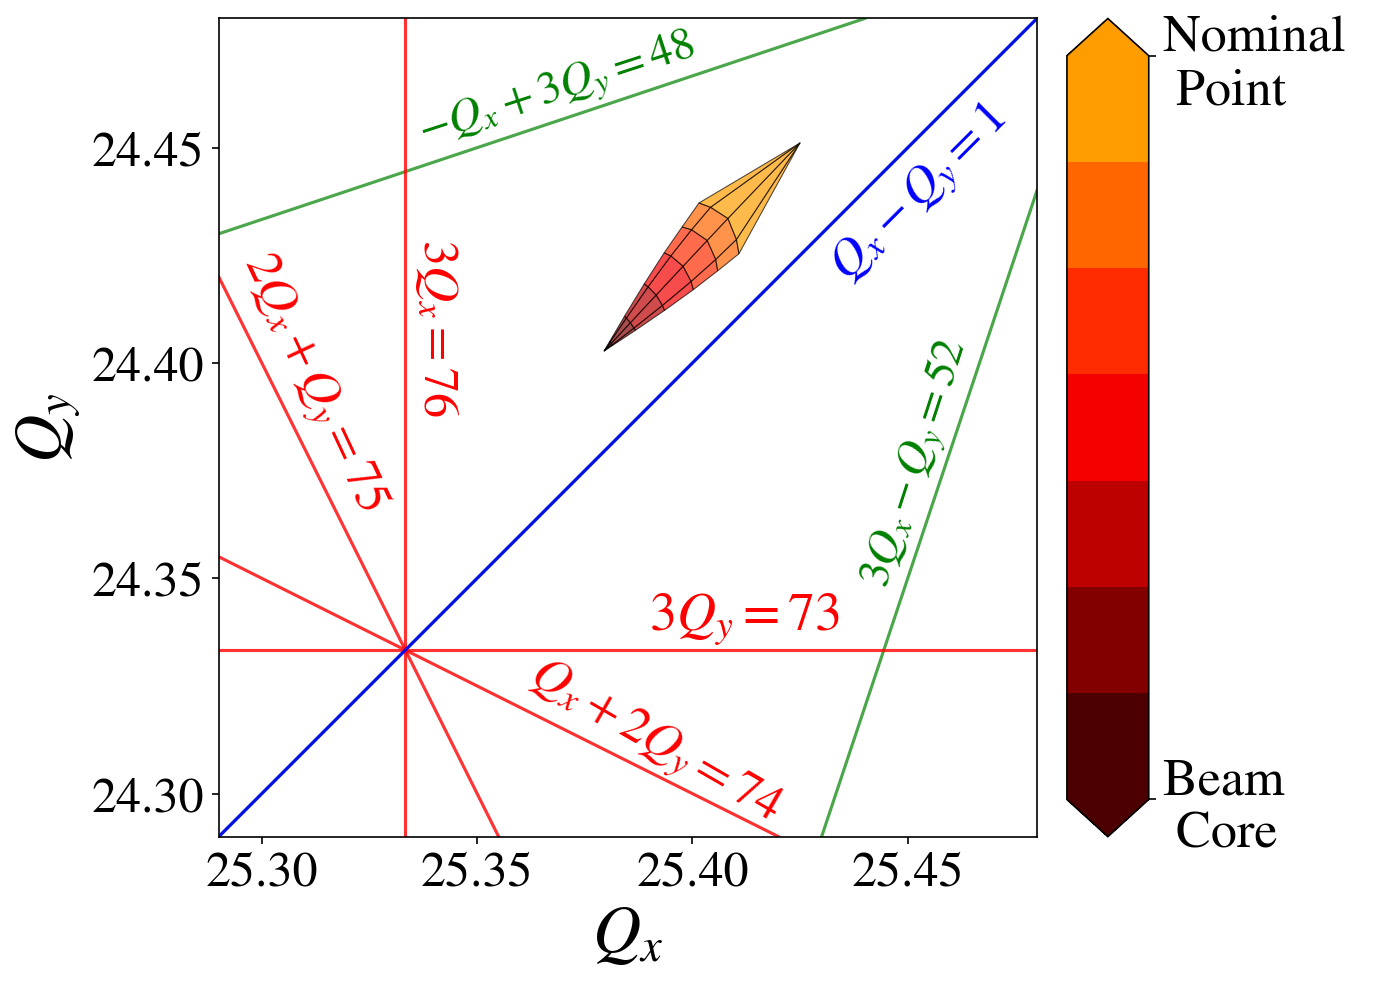
\includegraphics[width=\columnwidth]{chapter2/rrtdmid.png}
    \caption{Tune footprint for a Gaussian beam in the Recycler Ring at an intensity of 5e10 particles per bunch created with PySCRDT.}
    \label{fig:rrtdmid}
 \end{figure}

 Up until now, for this section the assumption $H_1=0$ holds. Nevertheless, in high-intensity particle accelerators there will be an interplay between the nonlinear Hamiltonian and the space charge potential. Ultimately, the terms $h_{jklm}$ and $G_{jklm}$ will dictate the perturbation to the linear Hamiltonian by their effective detuning. Therefore, the following Hamiltonian will describe the perturbation due to nonlinear elements in the circular lattice and due to space charge forces:
 \begin{multline}
    \label{eq:hfinal}
    H(J_x,\phi_x,J_y, \phi_y,\tilde{z})= 2\pi Q_x J_x + 2\pi Q_y J_y + \\
    \sum_{jklm} \left( h_{jklm}+G_{jklm} \right) \left( 2 J_x\right)^{\frac{j+k}{2}} \left( 2 J_y\right)^{\frac{l+m}{2}} e^{i\left[ \left( j-k \right)\left( \phi_x+\phi_{x0} \right)+ \left( l-m \right) \left( \phi_y+\phi_{y0} \right)\right]}.
\end{multline}